% knitr setup:

% maxwidth is the original width if it is less than linewidth
% otherwise use linewidth (to make sure the graphics do not exceed the margin)
\makeatletter
\def\maxwidth{ %
  \ifdim\Gin@nat@width>\linewidth
    \linewidth
  \else
    \Gin@nat@width
  \fi
}
\makeatother

\makeatletter
\newenvironment{kframe}{%
 \def\at@end@of@kframe{}%
 \ifinner\ifhmode%
  \def\at@end@of@kframe{\end{minipage}}%
  \begin{minipage}{\columnwidth}%
 \fi\fi%
 \def\FrameCommand##1{\hskip\@totalleftmargin \hskip-\fboxsep
 \colorbox{shadecolor}{##1}\hskip-\fboxsep
     % There is no \\@totalrightmargin, so:
     \hskip-\linewidth \hskip-\@totalleftmargin \hskip\columnwidth}%
 \MakeFramed {\advance\hsize-\width
   \@totalleftmargin\z@ \linewidth\hsize
   \@setminipage}}%
 {\par\unskip\endMakeFramed%
 \at@end@of@kframe}
\makeatother

\newenvironment{knitrout}{}{} % an empty environment to be redefined in TeX



% our setup:
\renewcommand{\P}[1]{\mathrm{P} \left( #1 \right)}
\newcommand{\Ps}[1]{\mathrm{P} \left( #1 \right)}
\newcommand{\Pwrt}[2]{\mathrm{P}_{#1} \left( #2 \right)}
\newcommand{\Pswrt}[2]{\mathrm{P}_{#1} \left( #2 \right)}

\newcommand{\pl}[1]{{\fontfamily{\sfdefault}\selectfont #1}}
\newtheorem{definition}{Definition}

\newcommand{\PRRV}[1]{P\left[#1\right]}
\newcommand{\PRRVwrt}[2]{P_{#1}\left[#2\right]}
\newcommand{\ve}[1]{\textbf{#1}}
\newcommand{\mc}[1]{\mathcal{#1}}
\newcommand{\al}{\alpha}
\renewcommand{\th}{\theta}
\renewcommand{\R}{\mathbb{R}}

% black text in example chunks
\definecolor{fgcolor}{rgb}{0, 0, 0}





\title{\pkg{ggdensity}: Improved Bivariate Density Visualization in R}
\author{by James Otto, David Kahle}

\maketitle
\abstract{
The \CRANpkg{ggdensity} \pl{R} package extends the functionality of \CRANpkg{ggplot2}
by providing more interpretable visualizations of bivariate density estimates using highest density regions (HDRs).
The visualizations are created via drop-in replacements for the standard \CRANpkg{ggplot2}
functions used for this purpose: \code{geom\_hdr()} for \code{geom\_density\_2d\_filled()}
and \code{geom\_hdr\_lines()} for \code{geom\_density\_2d()}.
These new geoms improve on those of \CRANpkg{ggplot2} by communicating the probabilities associated with the displayed regions.
Various statistically rigorous estimators are available,
as well as convenience functions \code{geom\_hdr\_fun()} and  \code{geom\_hdr\_fun\_lines()}
for plotting HDRs of user-specified probability density functions.
Associated geoms for rug plots and pointdensity scatterplots are also presented.
}




%%%%%
%%%%%%%%%%%%%%%%%%%%%%%%%%%%%%%%%%%%%%%%%%%%%%%%%%%%%%%%%%%%%%%%%%%%%%%%%%%%%%%%
\section{Introduction}\label{sec:introduction}

Density estimation is foundational to modern statistics.
Not only does it provide a theoretical basis for maximum likelihood estimation \citep{scott_multivariate_1992},
it is also an important tool in exploratory data analysis.
This is especially true for univariate data: histograms, frequency polygons, and kernel density estimates (KDEs) all visualize an estimated density.

With bivariate data, the situation is more complicated as the estimated density is a 3D surface, and there is a tendency to avoid 3D visualization in static graphics due to visual perception biases.
A more common strategy is to represent the surface using other geometric objects or aesthetics in a 2D plot, most commonly via contours of the density's level sets.
Typically the density is estimated with a KDE and the contours correspond to the level sets of an equally spaced mesh over $(0,M]$, where $M$ is the maximum of the estimated density's height (usually rounded to the closest "pretty" value).
We will refer to these contours as ordinate mesh density contours (OMDCs), and the corresponding graphics as traditional density contour plots or OMDC plots.
By ordinate, we mean the variable $z = f(x,y)$, or in general the last element of the graph of a function $f(\ve{x})$, which in this context represents density.

For example, the \CRANpkg{MASS} package documentation suggests using \code{MASS::kde2d()} with \\ \code{graphics::contour()}, which selects its level sets by calling \code{base::pretty()} on 10 such breaks over the $(0,M]$ ordinate range, and \CRANpkg{ggplot2}'s \code{geom\_density\_2d()} and \code{geom\_density\_2d\_filled()} do the same \citep{mass, wickham_ggplot2_2009, wilkinson_grammar_2005}.
Unfortunately, the resulting regions---those bounded by the OMDCs---cannot be immediately identified with corresponding probabilities, and are challenging to interpret in the best of cases.

Following \cite{hyndman_computing_1996}, we propose the use of highest density regions (HDRs) as replacements for density visualization based on OMDCs.
In a sense made rigorous in the next section, an HDR is the smallest region containing a certain percentage of the estimated distribution, e.g. 90\%.
An HDR contour is the boundary of this region.
HDRs are constructed by determining "good" cutoff values for the density, whereby cutoff values of the density we mean the ordinate values corresponding to the HDR contours
(i.e. the HDR contours are the level sets of these "good" cutoff values).
Unlike OMDCs, HDR contours' ordinate values are almost never equally spaced in the ordinate range, and computing them presents a number of practical and technical challenges.

In this article we introduce \CRANpkg{ggdensity}, a new \pl{R} package intended to address these challenges in facilitating the visualization of bivariate HDRs and related topics in the \CRANpkg{ggplot2} framework.
\CRANpkg{ggdensity} extends \CRANpkg{ggplot2} with a tight integration: instead of wrapping \CRANpkg{ggplot2} calls to return \code{ggplot} objects that are hard to modify, \CRANpkg{ggdensity} uses \CRANpkg{ggplot2}'s API to provide new extensible (geom, stat) pairs that behave in the way \CRANpkg{ggplot2} users have come to expect.
These new stats provide a range of density estimation options, as we describe in the next sections.

% The outline of the article is as follows.
% To contextualize our discussion, we begin with a motivating example that compares bivariate visualizations based on arbitrary density contours and HDRs, showing how arbitrary density contours are easily misinterpreted.
% We then present the technical definition of HDRs and discuss some of the challenges they pose.
% As it is easier to reason about such things in the 1d case, we start there before proceeding to the 2d case.
% With the technical and conceptual components established, we then present by example how different density estimation choices result in different HDRs and some of the practical implications of that fact.
% After presenting how \CRANpkg{ggdensity} can be used to visualize known densities, we present various applications and added features: contour line geoms (as opposed to filled contour geoms), pointdensity and rug geoms, and HDRs for arbitrary parametric models.
% We end with a brief discussion of related packages.




%%%%%
%%%%%%%%%%%%%%%%%%%%%%%%%%%%%%%%%%%%%%%%%%%%%%%%%%%%%%%%%%%%%%%%%%%%%%%%%%%%%%%%
\section{Motivating example}\label{sec:example}

We begin with a motivating example to show how traditional density contour plots can be misleading when exploring bivariate distributions.
The top left plot in Figure~\ref{fig:comparing_plots} is a scatterplot of simulated bivariate standard normal data whose distribution we want to visualize.
On the bottom left, we present the traditional way of visualizing the data's 2d distribution: a contour plot of slices of its estimated density (OMDCs).
The function that created this graphic, \code{geom\_density2d()} (alternatively \code{geom\_density\_2d()}), has been in \CRANpkg{ggplot2} since its inception.
It was modeled after a similar graphic made with base graphics using \code{MASS::kde2d()} with \code{contour()}.
In the top right is the filled contour version of the same plot, made with \code{geom\_density\_2d\_filled()}.
This type of plot was introduced in 2020 with \CRANpkg{ggplot2} version 3.3.2, which leveraged \CRANpkg{ggplot2}'s new dependency on \CRANpkg{isoband} that came in \CRANpkg{ggplot2} version 3.3.0 \citep{isoband}.
% \CRANpkg{isoband} implements a marching squares algorithm and associated data structures isolines and isobands that allow users to create polygons and lines associated with contour plots so that, for example, one can have regions with holes in them and that


In the bottom right is our proposed alternative, \code{ggdensity::geom\_hdr()}.
Each of the three contour plots show contours from the same estimated density surface, but the contours plotted by \code{geom\_hdr()} are HDR contours and are chosen to be inferentially relevant.
By default these are the smallest regions containing $50\%$, $80\%$, $95\%$, and $99\%$ of the estimated density.

Plotting the HDRs results in a significantly more interpretable graphic that conveys more information than equally spaced density contours.
To make a more direct comparison, in Figure~\ref{fig:comparing_plots-2} we superimpose the HDR contours onto the filled traditional density contour plot in the top right of Figure~\ref{fig:comparing_plots}.
The result reveals that nearly 20\% of the estimated distribution is outside the lowest OMDC.
Consequently, we would expect almost 1 out of every 5 observations to fall outside the traditional density contour plot.

This is somewhat of a cautionary tale: while the contours seen in the bottom left and top right plots of Figure~\ref{fig:comparing_plots} do seem to communicate some information to the viewer, it's hard to say exactly what that information is.
And worse: it seems surprisingly easy to draw wrong conclusions.
Upon scrutiny, the overall OMDC strategy seems suspect as a general purpose tool for visualizing where the probability mass of a bivariate distribution resides as it focuses exclusively on the density and ignores the region over which that density extends.
On the other hand, with HDRs one immediately understands where the majority of the observed data lie and
roughly how much data lies in each region.
It is not possible to achieve these insights with traditional density contour plots, since equivalent interpretations require double integrals of the estimated density.





\begin{knitrout}
\definecolor{shadecolor}{rgb}{1, 1, 1}\color{fgcolor}\begin{widefigure}[h!]

{\centering 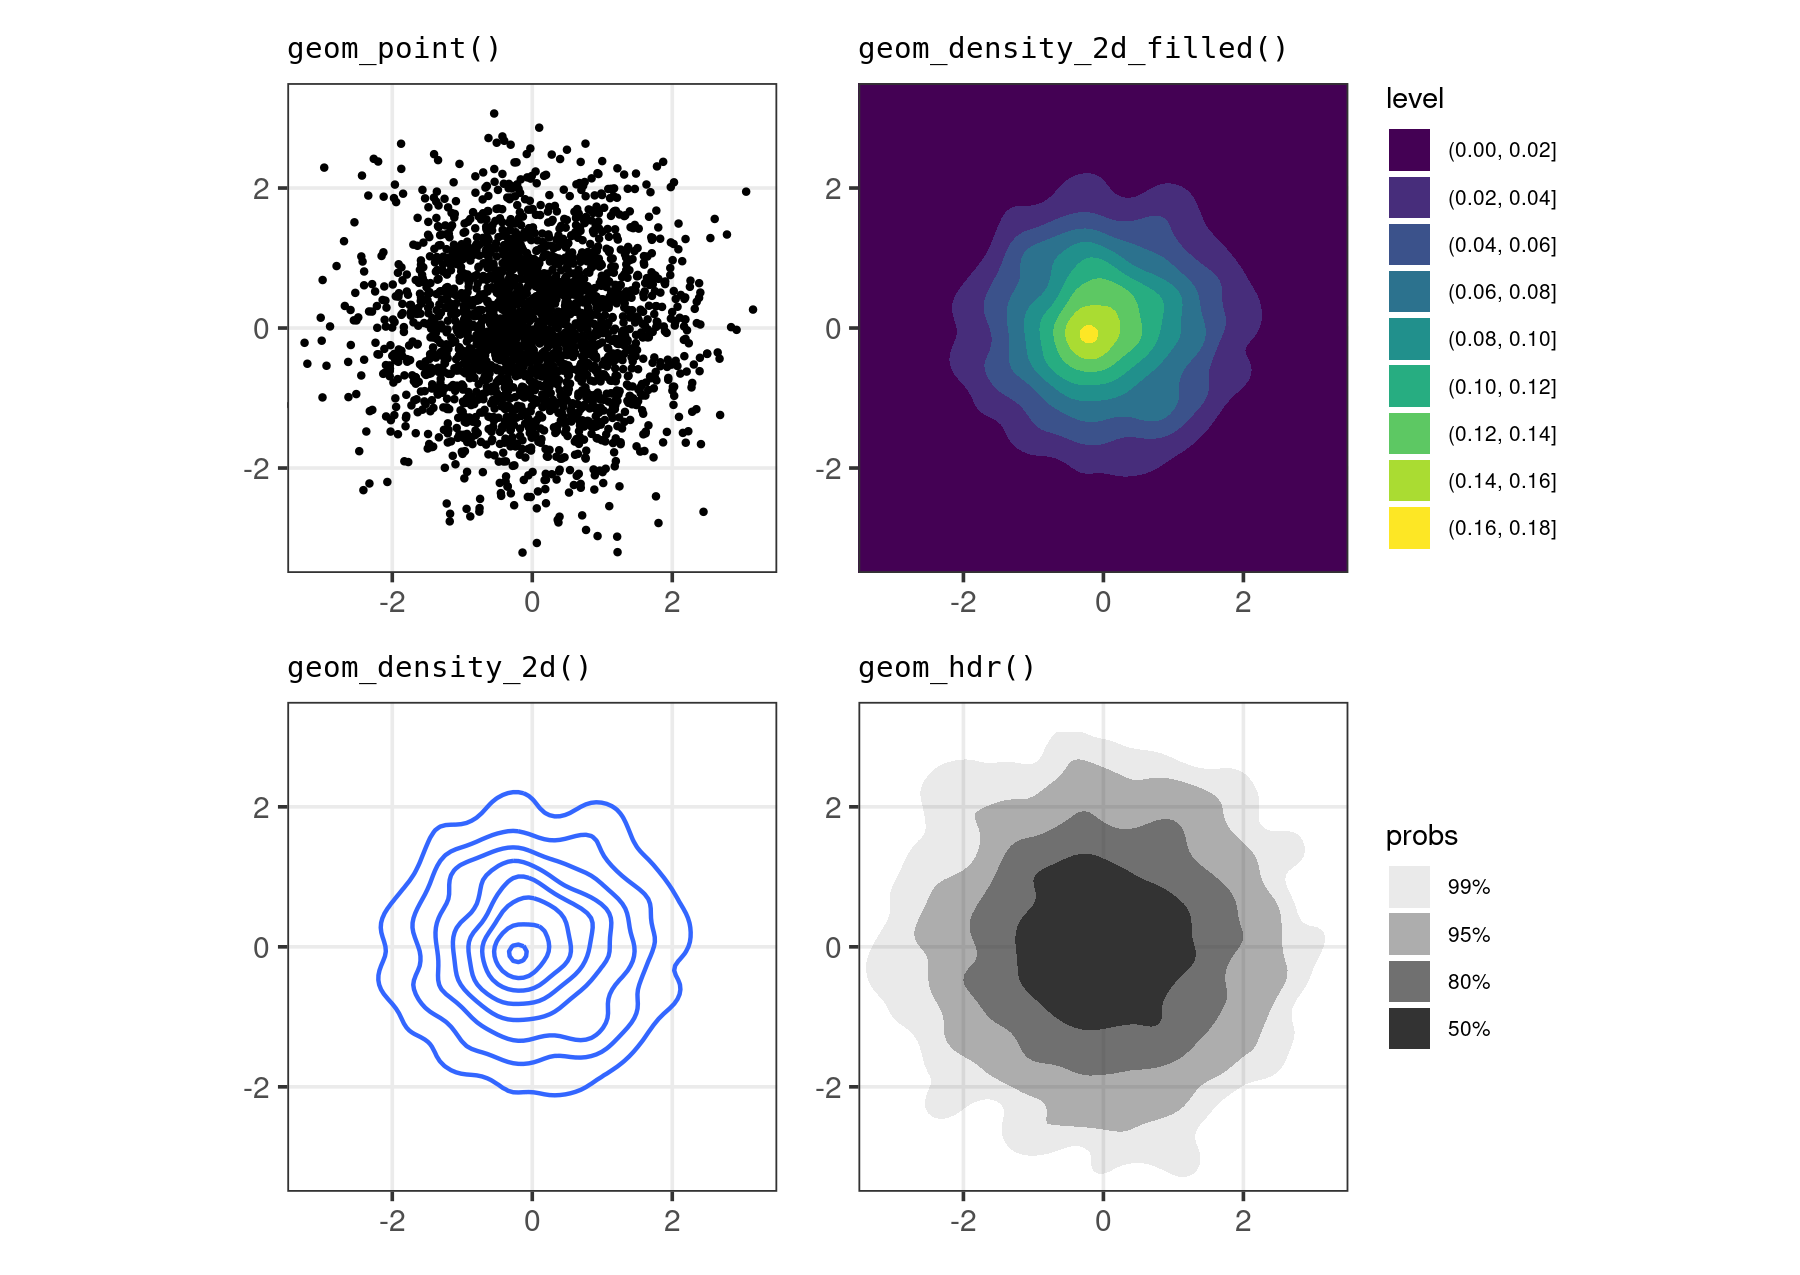
\includegraphics[width=\maxwidth]{figures/comparing_plots-1}

}

\caption{Comparing various geoms on a bivariate standard normal sample of size $n = 2500$.}\label{fig:comparing_plots}
\end{widefigure}

\end{knitrout}



\begin{knitrout}
\definecolor{shadecolor}{rgb}{1, 1, 1}\color{fgcolor}\begin{widefigure}[h!]

{\centering 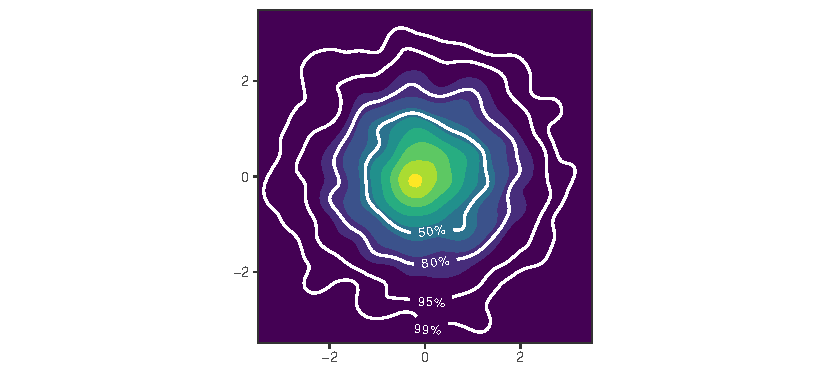
\includegraphics[width=\maxwidth]{figures/comparing_plots-2-1}

}

\caption{\code{geom\_density\_2d\_filled()} and \code{geom\_hdr()} (white) from Figure~\ref{fig:comparing_plots}, showing that the traditional density contour plots can mislead: nearly 20\% of the estimated distribution falls outside the lowest OMDC. Labels generated with \CRANpkg{geomtextpath} \citep{geomtextpath}.}\label{fig:comparing_plots-2}
\end{widefigure}

\end{knitrout}



\pagebreak


%%%%%
%%%%%%%%%%%%%%%%%%%%%%%%%%%%%%%%%%%%%%%%%%%%%%%%%%%%%%%%%%%%%%%%%%%%%%%%%%%%%%%%
\section{Highest density regions}\label{sec:hdrs}

More formally, following \cite{hyndman_computing_1996}  we adopt the following definition of highest density regions (HDRs):

\begin{definition}\label{def:HDR}
Let $f(\ve{x})$ be the probability density function (PDF) of a random vector $\ve{X} \in \R^{p}$ and $\al \in (0,1)$.
For any constant $c \in \R$ define $\mc{R}_{f}(c) = \{\ve{x} \in \R^{p}: f(\ve{x}) \geq c\}$ to be the subset of the sample space of $\ve{X}$ with density at least $c$. The $100(1 - \al)\%$ HDR of $\ve{X}$ is the subset $\mc{R}_{f}(f_{\al})$, where $f_{\al}$ is the largest constant $c$ such that $p_{f}(c) := \PRRVwrt{f}{\ve{X} \in \mc{R}_f(c)} \geq 1 - \al$. When $f(x)$ is clear, we will simplify this to $\mc{R}_{\al} = \mc{R}_{f}(f_{\al})$.
\end{definition}

Note that $p_{f}(c)$ is non-increasing in $c$.
Intuitively, we see that as $c$ gets bigger the region where $f(\ve{x}) \geq c$ shrinks
(or possibly remains unchanged),
and so the probability of the region gets correspondingly smaller (or at least can't get bigger).
% Alternatively, as $c$ decreases, the region grows and the probability also grows.
% (Removed as it is redundant and it is difficult to respect possibility of constancy in a readable way)
$f_{\al}$ is the largest point at which this probability is at least $1 - \al$.
We revisit this in the next section.

Of course, in practice we are given data $\ve{x}_{1}, \ldots, \ve{x}_{n}$, ideally a random sample from $f(\ve{x})$, and we need to estimate the population HDRs.
The problem of estimating HDRs, and more generally density contour estimation, has been widely studied and several estimators have been proposed.
Estimators generally fall in one of three classes: plug-in estimators \citep{rigollet_optimal_2009, cadre_kernel_2006}, excess mass estimators \citep{muller_excess_1991, polonik_measuring_1995}, and convex contour estimators \citep{hartigan_estimation_1987}.
In this work we focus exclusively on plug-in estimators of HDRs
due to their straightforward interpretation and implementation.
These estimators are of the form $\widehat{\mc{R}}_{\al} = \widehat{\mc{R}}_{f}(f_{\al}) := \mc{R}_{\hat{f}}(\hat{f}_{\al})$ for some PDF estimate $\hat{f}(\ve{x})$ of $f(\ve{x})$, where $\hat{f}_{\al}$ is the largest value $c$ such that $\hat{p}_{f}(c) := p_{\hat{f}}(c) = \PRRVwrt{\hat{f}}{\ve{X} \in \mc{R}_{\hat{f}}(c)} \geq 1 - \al$.

% \begin{definition}\label{def:sample_HDR}
% Let $\hat{f}(\ve{x})$ be a PDF estimate of $f(\ve{x})$ and $\al \in (0,1)$.
% The $100(1 - \al)\%$ sample HDR corresponding to $\hat{f}(\ve{x})$ is the set  $\widehat{\mc{R}}_{f}(f_{\al}) := \mc{R}_{\hat{f}}(\hat{f}_{\al})$, the $100(1 - \al)\%$ HDR of the distribution $\hat{f}(\ve{x})$. In particular, $\hat{f}_{\al}$ is the largest value $c$ such that $\hat{r}_{f}(c) := r_{\hat{f}}(c) := \PRRVwrt{\hat{f}}{\ve{X} \in \mc{R}_{\hat{f}}(c)} \geq 1 - \al$.
% \end{definition}


% Recently, methods of HDR estimation have been proposed for directional data and densities on smooth manifolds \citep{saavedra-nieves_nonparametric_2021-1, cholaquidis_level_2022}.
% For an application of HDR estimation for identifying and visualizing hot-spots of COVID-19 cases in the United States, see \cite{saavedra-nieves_nonparametric_2021-1}.

Thus, plug-in HDR estimators estimate population HDRs with the HDRs of estimated densities.
As there are many ways to estimate a density, both parametric and nonparametric,
one can arrive at many different HDR estimates with the same data and probability mass $1 - \al$,
and different choices confer advantages and disadvantages.
We revisit this notion in \nameref{sec:hdr-methods} using \CRANpkg{ggdensity} after explaining how such estimates can be computed.

Before addressing that topic, it is worth reflecting on another aspect that makes HDRs so special: their size. While HDRs are primarily of interest because their corresponding probabilities are immediately interpretable, they are also important because they are the smallest such sets that contain their probabilities.

For any continuous distribution, there are an infinite number of different regions in its support that contain probability at least $1 - \al$.
The standard normal distribution provides a simple univariate example.
If $\Phi^{-1}(x)$ is the quantile function of the standard normal distribution and $0 \leq l < u \leq 1$ with $u - l = 1 - \al$,
any interval of the form $[\Phi^{-1}(l), \Phi^{-1}(u)]$ contains probability exactly $1-\al$, and indeed these are all such intervals that do.
This is because $\PRRV{\Phi^{-1}(l) \leq Z \leq \Phi^{-1}(u)} = \PRRV{Z \leq \Phi^{-1}(u)} - \PRRV{\Phi^{-1}(l) \leq Z} = \Phi(\Phi^{-1}(u)) - \Phi(\Phi^{-1}(l)) = u - l = 1 - \al$.
Setting $1 - \al = .95$, we can choose
$l = 0$, $u = .95$ yielding the interval $(-\infty, 1.645]$.
We can find similar intervals with other choices of $l, u$:
$[-2.326, 1.751]$;
$[-2.054, 1.881]$;
$[-1.881, 2.054]$;
$[-1.751, 2.326]$; and
$[-1.645, \infty)$,
all of which contain 95\% probability.
% $l = .01$, $u = .96$ yielding $[-2.326, 1.751]$;
% $l = .02$, $u = .97$ yielding $[-2.054, 1.881]$;
% $l = .03$, $u = .98$ yielding $[-1.881, 2.054]$;
% $l = .04$, $u = .99$ yielding $[-1.751, 2.326]$;
% $l = .05$, $u = 1$ yielding $[-1.645, \infty)$;

However, all intervals are typically not equally preferable: if we are interested in summarizing the normal distribution with a set of probability $1 - \al$, we typically want to provide the smallest such set.
The intervals above have lengths $\infty$, 4.08, 3.93, 3.93, 4.08, and $\infty$.
As is well-known, if we want the smallest interval, we use $[\Phi^{-1}(\al/2), \Phi^{-1}(1-\al/2)] = [-1.96, 1.96]$ as the interval bounds, with the interval length of 3.92.
This interval corresponds to the region where the density exceeds $f_{\al} = \phi(\Phi^{-1}(\al/2))$;
and as such meets the definition of an HDR.

This is a general feature of HDRs: whether in one or many dimensions, they constitute the smallest regions containing their corresponding probabilities, a fact seen from the following measure-theoretic argument. For some $f(\ve{x})$, $\al \in [0, 1]$, and an associated HDR $\mc{R}_{\al}$, let $\eta = \PRRV{\ve{X} \in \mc{R}_{\al}}$. While $\eta$ may be equal to $1 - \al$, in some cases it may be more, for instance in the case of the uniform distribution. % Suppose $\mc{A}$ is another subset of the sample space of $\ve{X}$ with probability $\eta$. Then
Suppose $\mc{A}$ is a subset of the sample space of $\ve{X}$ with probability $\xi \geq \eta$ such that $\mc{A} \setminus \mc{R}_{\al}$ is non-null, i.e.  $\mc{A}$ and $\mc{R}_{\al}$ are not the same set. Then
$$
\eta = \PRRV{\ve{X} \in \mc{R}_{\al}}
= \int_{\mc{R}_{\al}}f(\ve{x})d\ve{x}
= \int_{\mc{R}_{\al} \cap \mc{A}}f(\ve{x})d\ve{x} + \int_{\mc{R}_{\al} \setminus \mc{A}}f(\ve{x})d\ve{x}.
$$
Similarly,
$$
\xi = \PRRV{\ve{X} \in \mc{A}}
= \int_{\mc{R}_{\al} \cap \mc{A}}f(\ve{x})d\ve{x} + \int_{\mc{A} \setminus \mc{R}_{\al}}f(\ve{x})d\ve{x}.
$$
Since $\xi \geq \eta$,
$$
\int_{\mc{A} \setminus \mc{R}_{\al}}f(\ve{x})d\ve{x}
\geq
\int_{\mc{R}_{\al} \setminus \mc{A}}f(\ve{x})d\ve{x}
$$
By the definition of $\mc{R}_{\al}$, $f_{\al} > f(\ve{x})$ over $\mc{A} \setminus \mc{R}_{\al}$ and $f(\ve{x}) \geq f_{\al}$ over $\mc{R}_{\al}$.
Thus,
$$
  f_{\al} m(\mc{A} \setminus \mc{R}_{\al})
  = \int_{\mc{A} \setminus \mc{R}_{\al}}f_{\al}d\ve{x}
  > \int_{\mc{A} \setminus \mc{R}_{\al}}f(\ve{x})d\ve{x}
  \geq \int_{\mc{R}_{\al} \setminus \mc{A}}f(\ve{x})d\ve{x}
  \geq \int_{\mc{R}_{\al} \setminus \mc{A}}f_{\al}d\ve{x}
  = f_{\al} m(\mc{R}_{\al} \setminus \mc{A}),
$$
where $m$ denotes the Lebesgue measure of the given set, its size. Thus $m(\mc{A}\setminus \mc{R}_{\al}) > m(\mc{R}_{\al} \setminus \mc{A})$ and consequently $m(\mc{A}) > m(\mc{R}_{\al})$.

The minimality of HDRs comes with a few trade-offs.
First, there may be other regions of the sample space with probability between $1 - \al$ and $\eta$, the nominal and actual probabilities of the HDRs respectively, that are smaller than the HDR.
This can happen in cases where the PDF is constant on some set of positive measure so that $p_{f}(c)$ jumps discontinuously over $1 - \al$.
The $100(1-\al)$\% quantile interval of the $\mbox{Unif}(0,1)$ distribution, $[\al/2, 1-\al/2]$, illustrates this, for instance; it contains probability exactly $1-\al$ and is of length $1-\al$.
By contrast, the $100(1-\al)$\% HDR for the uniform distribution is $\mc{R}_{\al} = [0,1]$ for any $\al$, contains 100\% of the distribution, and is of length $1$.
While this is a rare circumstance when using density estimators, it does occur when constructing HDRs from histogram density estimates --
they always contain more than nominal probability.
The second trade-off is that HDRs are only connected sets for all $\al$ if the distribution is unimodal.
This is rarely the case for density estimators, so it is common for the lowest probability HDRs, the smallest sets, to be disconnected: two or more intervals in 1D and unions of blobs in 2D.
A third challenge is that HDRs are non-trivial to compute. It is to this challenge that we now turn.


% As mentioned previously, this is known as the plug-in estimator of $\mc{R}_f(f_{\alpha})$\textemdash it results from "plugging in" an estimate $\hat{f}$.
% \placeholder{Add references for details such as consistency of plug-in estimates of HDRs (specifically for "well-behaved" $\hat{f}$).}
% The sample HDR is defined for any estimate of a density function, $\hat{f}$.
% For different choices of $\hat{f}$, the corresponding sample HDRs have different properties that can be both advantageous and disadvantageous.
% We will explore this later, comparing visualizations of sample HDRs based on KDEs, parametric estimators, and others forms of density estimation.

% \placeholder{Not sure where to include these thoughts:}
% In addition to the proposed use in data visualization, HDRs have many applications.
% The most well-known of which is the highest posterior density region in Bayesian analysis \placeholder{(ref for HPD)}.
% \placeholder{Also maybe used to find prediction intervals?}


%%%%%
%%%%%%%%%%%%%%%%%%%%%%%%%%%%%%%%%%%%%%%%%%%%%%%%%%%%%%%%%%%%
\section{Computing highest density regions}\label{sec:computing}


% Implementation-wise, this is facilitated by the ggproto system of object oriented programming which allows for the development of \CRANpkg{ggplot2} extensions capable of being used alongside its intuitive API and extensive toolset.


% There are many other \CRANpkg{ggplot2} extensions which implement summary-style visualizations based on statistical methods,
% \placeholder{list out some example packages: \CRANpkg{ggstatsplot}, \CRANpkg{ggdist}, \CRANpkg{see}, \CRANpkg{gglm}}.


\CRANpkg{ggdensity} enables the computation and visualization of 2D HDRs based on various plug-in estimators, extending the functionality of \CRANpkg{ggplot2}.
% To do so, it must solve the optimization problem that maximizes $c$ subject to the constraint that $p_{\hat{f}}(c) \geq 1 - \al$.
% Attempting to find a closed form for $c$, and therefore to some extent the HDR $\widehat{\mc{R}}_{f}(f_{\al})$, is impractical in almost all cases.
% Therefore, to calculate sample HDRs we must utilize numerical techniques for all but the simplest choices of  $\hat{f}$.
% The strategy used in \CRANpkg{ggdensity} is the subject of this section.
In order to understand how HDRs are computed in two dimensions, we find it helpful to first illustrate the process in one dimension.


%%%%%
%%%%%%%%%%%%%%%%%%%%%%%%%%%%%%%%%%%%%%%%%%%%%%%%%%%%%%%%%%%%
\subsection{Computing HDRs in one dimension}\label{sec:hdr1d}

Consider the challenge of computing the 95\% HDR of the standard normal distribution with PDF $f(x) = \phi(x)$.
One way to do this might be to fix a $c$, determine the interval $[l,u]$ over which $\phi(x) \geq c$, integrate $\phi(x)$ over $[l,u]$, and move $c$ up or down depending on whether the interval contains too much or too little probability.
$l$ and $u$, the boundaries of the interval where $\phi(x) \geq c$, can be determined numerically or algebraically from $\phi(x) = c$, and the integral can be done via numerical integration.
$f_{\al}$, the special $c$ that provides $1 - \al$ probability, can also be determined numerically in many ways.

Unfortunately, this method doesn't scale well.
In general, the set $\mc{R}_{f}(c)$ will not be a simple interval as in the normal case.
It will instead be a union of an unknown number of intervals whose boundaries are unknown and hard to determine.
Once known, numerical integration can be relied upon to determine the integral, but only easily in one dimension.
In two or more dimensions, the situation is significantly more complex.
The region $\mc{R}_{f}(c)$ is implicitly described, and therefore some form of grid-based approximation would be required before numerical integration could be applied.
Notice that there are essentially two hard problems here: computing $\mc{R}_{f}(c)$, in the sense of determining a useful description of it, and computing $p_{f}(c)$.

% challenge here really depends on the ability to compute $p_{f}(c)$ for a given $c$; the ability to compute the region over which the . If that were easy, then the computation would be vastly simplified: a simple univariate root finder would work, even in the multivariate case. Unfortunately, it is not immediately obvious how to compute $$p_{f}(c)$

The basic idea used by \CRANpkg{ggdensity} is simple: discretize and compute. In the univariate case, the fundamental algorithm is this:
\begin{enumerate}
\item Evaluate $f(x)$ on a regular mesh $\{x_{i}: i = 1, \ldots N\}$ to obtain $f_{i} = f(x_{i})$ over some interval nominally larger than the support of the data to create a table with rows $(x_{i}, f_{i})$ for $i = 1, \ldots, N$.
\item Normalize the points into a discrete distribution $p_{i} = f_{i} / \sum_{i}f_{i}$ to create the table $(x_{i}, f_{i}, p_{i})$.
\item Sort the $N$ rows of the table $(x_{i}, f_{i}, p_{i})$ by $p_{i}$ in decreasing order to obtain $(x_{(i)}, f_{(i)}, p_{(i)})$.\footnote{This is actually the opposite of order statistics notation: here $p_{(1)}$ is the \emph{largest} probability of the discretized distribution, and $x_{(1)}$ is the corresponding $x_{i}$ value.}
\item Compute the cumulative sum $a_{(k)} = \sum_{i=1}^{k} p_{(i)}$  to create the table $(x_{(i)}, f_{(i)}, p_{(i)}, a_{(i)})$.
\item Estimate $f_{\al}$ with the first $f_{(i)}$ such that $a_{(i)} \geq 1 - \al$.
\end{enumerate}
The point masses $p_{i}$ of the discrete approximation are in fact the areas of the rectangles of a Riemann (i.e. piecewise constant) approximation to $f(x)$ collapsed to individual points: they approximate the probability over a range such as $[x_{i}-\delta/2, x_{i}+\delta/2]$, where $\delta$ is the resolution of the mesh. Just as Riemann approximations converge to the true value of the integral under very minor conditions on $f(x)$, arbitrarily accurate approximations to $f_{\al}$ can be obtained by setting $N$ suitably large. Because of this, we will refer to approximating $f_{\al}$ as ``computing'' $f_{\al}$ instead of estimating it, and our notation will not reflect the fact that it is an approximated quantity.

With $f_{\al}$ in hand, the HDR can be approximated in any of a number of ways that are practically equivalent for sufficiently large $N$. The easiest is to simply union of intervals $[x_{i}-\delta/2, x_{i}+\delta/2]$ such that $f_{i} \geq f_{\al}$. Figure~\ref{fig:hdr-1d-1} provides an illustration of the process using a very coarse mesh to emphasize the process.

\vspace{-1em}

\begin{knitrout}
\definecolor{shadecolor}{rgb}{1, 1, 1}\color{fgcolor}\begin{figure}[h!]

{\centering 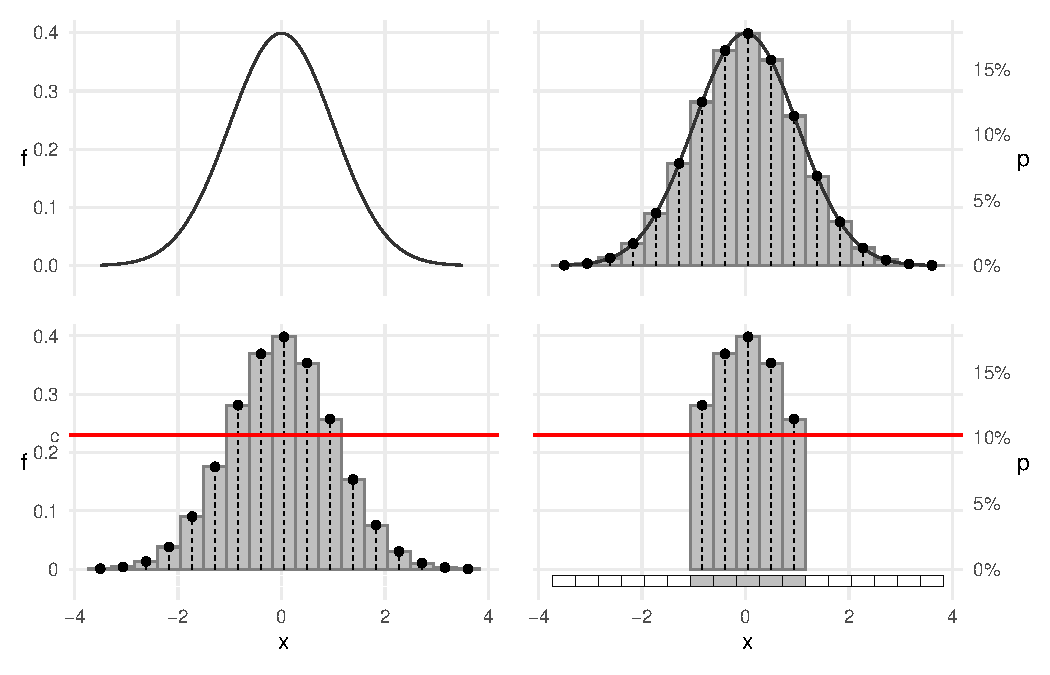
\includegraphics[width=\maxwidth]{figures/hdr-1d-1-1}

}
\caption{$p_{f}(c)$ and $\mc{R}_{f}(c)$ are computed by discretizing the density $f(x)$, determining the probabilities with densities above $c$, and constructing HDRs as unions of intervals.
In this illustration, $c = .23$, yielding $p_{f}(c) = .763$.
}\label{fig:hdr-1d-1}
\end{figure}

\end{knitrout}

\newpage


\begin{knitrout}
\definecolor{shadecolor}{rgb}{1, 1, 1}\color{fgcolor}\begin{figure}[h!]

{\centering 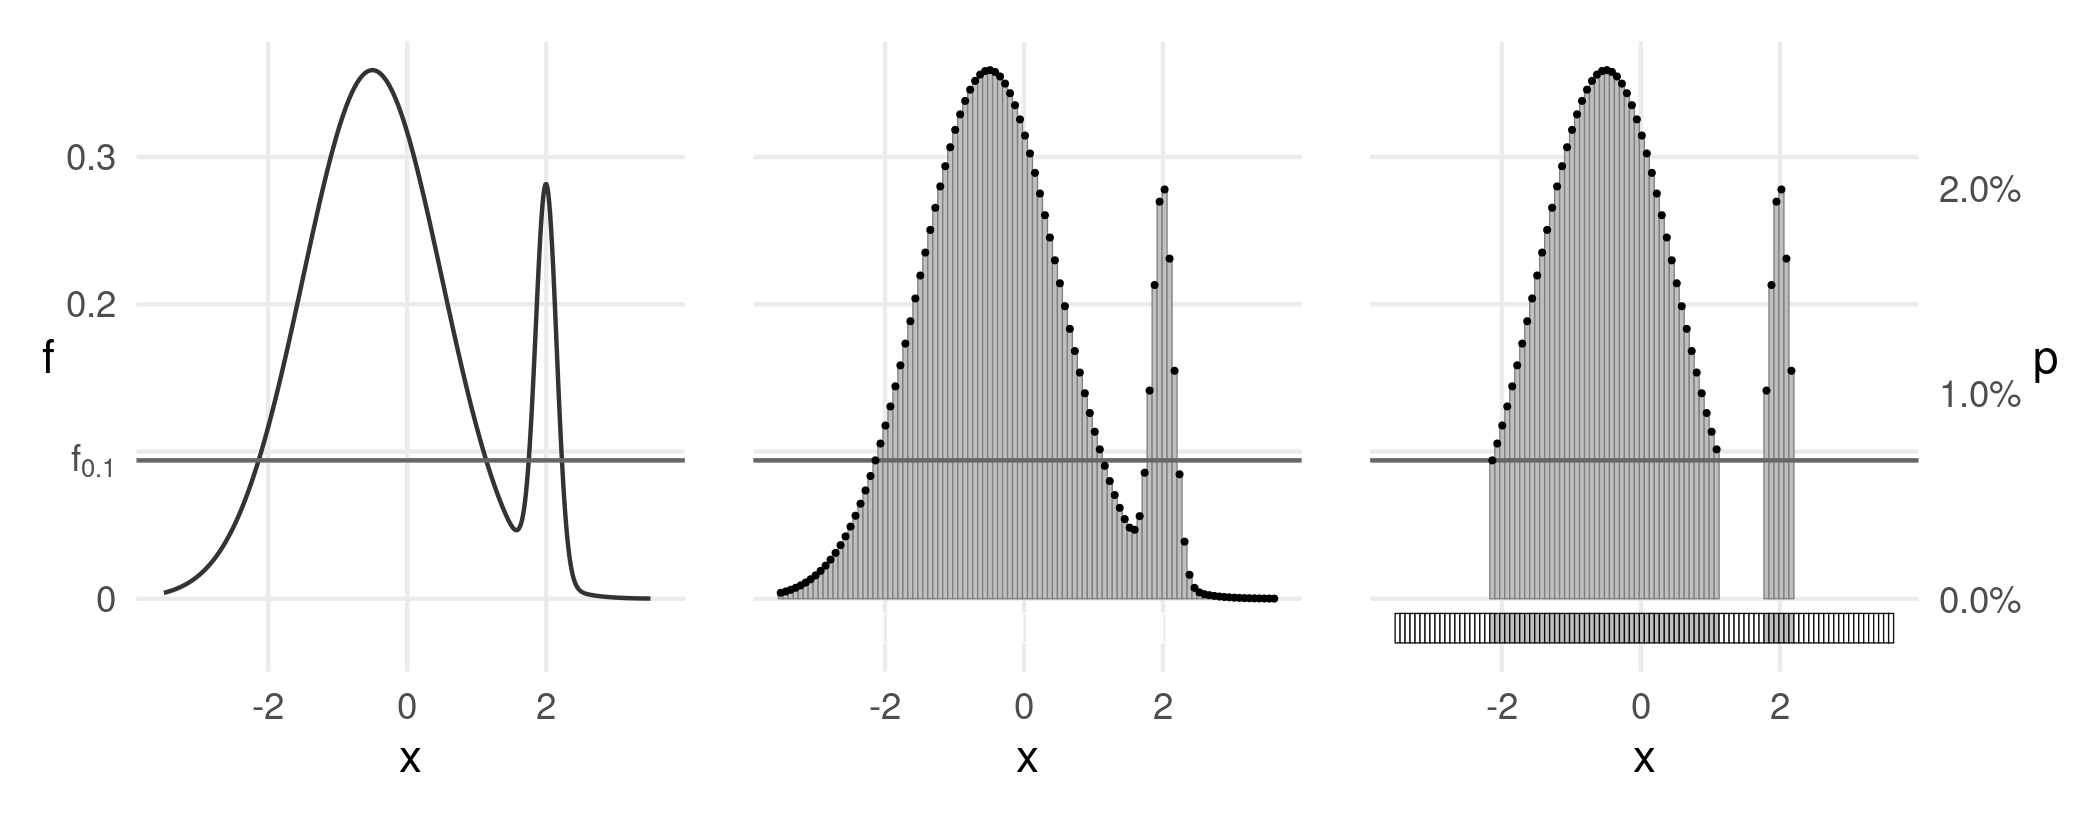
\includegraphics[width=\maxwidth]{figures/hdr-1d-2-1}

}

\caption{As the mesh size $N$ grows, the HDR approximation improves for any $f(x)$. Here $N = 100$ and the 90\% HDR is illustrated.}\label{fig:hdr-1d-2}
\end{figure}

\end{knitrout}

$N$ governs the accuracy of the approximation of $p_{f}(c)$ and the accuracy and resolution of $\mc{R}_{f}(c)$ in the resulting plot. Consequently, a reasonably large number is desired: \CRANpkg{ggdensity} defaults this parameter to $N = 512$ in \code{geom\_hdr\_rug()}.
Figure~\ref{fig:hdr-1d-2} illustrates a more complicated example with a bimodal $f$ where $N = 100$ is used so that it is still possible to see the approximation.

Two adjustments are needed to fully operationalize 1D HDRs for data: using an approximation $\hat{f}(x)$ in place of $f(x)$ and plotting several HDRs. Fortunately, both of these are easy. In practice density estimator implementations usually return their estimates as values of the function $\hat{f}_{i} = \hat{f}(x_{i})$ on a mesh, not as some analytic expression. Such is the case for \code{stats::density()}, for example, which accepts a univariate vector and returns its estimated density at $N = 512$ points on a regular mesh a little larger than the data. Similarly, computing several HDRs at once requires virtually no added computational expense: HDRs are nested regions, so to find several HDRs simply continue looking down the list of accumulated probabilities $a_{(i)}$ until the desired probabilities are reached. This is illustrated in Figure~\ref{fig:hdr-1d-3}.

% The process for numerically approximating $\hat{f}_{\alpha}$ when we have sample data is therefore very similar, this is illustrated below in Figure~\ref{fig:hdr-1d-3}.
% Figure~\ref{fig:hdr-1d-3} substitutes the KDE $\hat{f}(x)$ for the known $f(x)$,
% finding $\hat{f}_{\alpha}$ and the corresponding $\mc{R}_{\hat{f}}(\hat{f}_{\alpha})$ via the same procedure of choosing $\hat{f}_{\alpha}$ to be as large as possible while $\Pwrt{\hat{f}}{\mc{R}_{\hat{f}}(\hat{f}_{\alpha})} \geq 1 - \alpha$ for our rescaled discrete approximation.


\begin{knitrout}
\definecolor{shadecolor}{rgb}{1, 1, 1}\color{fgcolor}\begin{figure}[h!]

{\centering 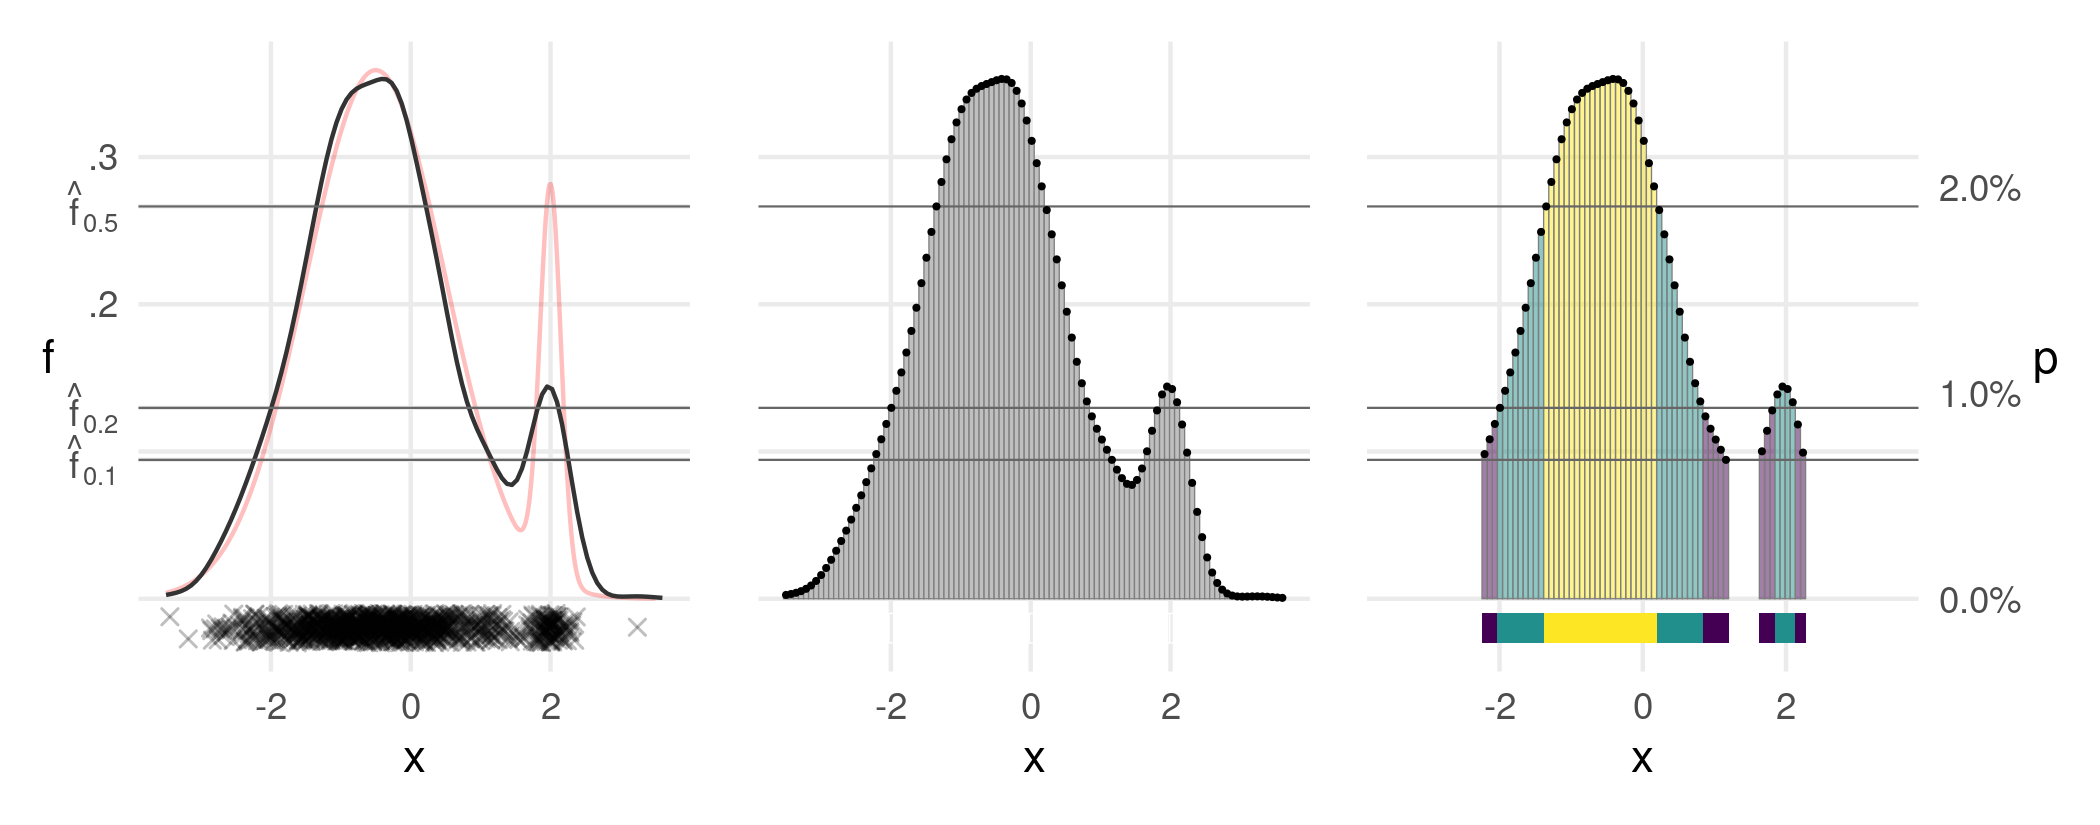
\includegraphics[width=\maxwidth]{figures/hdr-1d-3-1}

}

\caption{Computing several HDRs can be done with no added computational complexity, since the regions are nested. Here the 50\%, 80\%, and 90\% HDRs $\widehat{\mc{R}}_{\al}$ are illustrated using an estimated density based on $n = 1000$ draws.}\label{fig:hdr-1d-3}
\end{figure}

\end{knitrout}



% Included in Figure~\ref{fig:hdr-1d-1} are four plots illustrating the numerical procedure of approximating
% $f_{\al}$ and the corresponding $\mc{R}_f(f_{\al})$ for $\al = .5, .2, .05, .01$ for the standard normal distribution, corresponding to 50\%, 80\%, 95\%, and 99\% HDRs.
% On the left, we plot the standard normal density, $f(x) = \phi(x)$.
% In the middle, we show a discrete approximation of $f(x)$ and visualize the approximation to $p_{f}(.25)$ as the sum of the probabilities over $.25$.
% Moving from the density to probability scale is handled behind the scenes
% Here $.25$ was ar
% To compute the probability, we sum the probabilities associated with the non-dotted lines after a rescaling to ensure our approximation is a valid probability mass function.
% On the right, we plot the approximated $f_{\al}$ values and their associated HDRs.
% Each of these values were chosen to be as large as possible with the approximated $\Pwrt{f}{\mc{R}_f(f_{\al})} \geq 1 - \al$.
% In practice this is implemented by sorting each point on the approximation in descending order by its associated probability mass and computing the cumulative sum of the probabilities,
% setting $f_{\al}$ as the largest value with corresponding cumulative sum greater than or equal to $1 - \al$.


% The process for numerically approximating $\hat{f}_{\alpha}$ when we have sample data is very similar,
% this is illustrated below in \ref{fig:hdr-1d-sample}.
% Now, we have substituted the KDE $\hat{f}$ for the known $f$,
% finding $\hat{f}_{\alpha}$ and the corresponding $\mc{R}_{\hat{f}}(\hat{f}_{\alpha})$ via the same procedure of choosing $\hat{f}_{\alpha}$ to be as large as possible while $\Pwrt{\hat{f}}{\mc{R}_{\hat{f}}(\hat{f}_{\alpha})} \geq 1 - \alpha$ for our rescaled discrete approximation.


% Notice that the definition of the HDR handles the improbable scenario in which $\hat{f}(x_1) = \hat{f}(x_2) = \hat{f}_{\alpha}$ for $x_1$ and $x_2$ on the discrete approximation.
% It will always be the case that $x_1, \; x_2 \in \mc{R}_{\hat{f}}(\hat{f}_{\alpha})$ as $\Pwrt{\hat{f}}{\mc{R}_{\hat{f}}(\hat{f}_{\alpha})}$ is allowed to exceed $1 - \alpha$.
% Also, it is important to point our that this numerical procedure handles disconnected HDRs, as we will see in examples in later sections.
% As a final note, the discretizations in figures \ref{fig:hdr-1d} and \ref{fig:hdr-1d-sample} are much lower resolution than the approximations used by \CRANpkg{ggdensity}\textemdash
% they were chosen to better illustrate the process of finding the cutoff values.


\pagebreak

%%%%%
%%%%%%%%%%%%%%%%%%%%%%%%%%%%%%%%%%%%%%%%%%%%%%%%%%%%%%%%%%%%
\subsection{Finding HDRs in two dimensions}\label{sec:hdr2d}

The procedure for finding $\mc{R}_{\al}$ for bivariate data is very similar to the univariate case.
The basic idea behind the computation of HDRs in \CRANpkg{ggdensity} is again to discretize $f(\ve{x}) = f(x,y)$ and compute. The fundamental algorithm is this:
\begin{enumerate}
\item Evaluate $f(x,y)$ on a fine mesh $\{(x_{i},y_{j}): i = 1, \ldots N_{x}, j = 1, \ldots N_{y}\}$ to obtain $f_{ij} = f(x_{i},y_{j})$ over some rectangular region nominally larger than the support of the data to create a table $(x_{i}, y_{j}, f_{ij})$ for $i = 1, \ldots, N_{x}$ and $j = 1, \ldots, N_{y}$. In practice, we usually use $N = N_{x} = N_{y}$.
\item Normalize the points into a discrete distribution $p_{ij} = f_{ij} / \sum_{i,j}f_{ij}$ to obtain the table $(x_{i}, y_{j}, f_{ij}, p_{ij})$.
\item Sort the rows of the table by $p_{ij}$ in decreasing order to obtain $(x_{(k)}, y_{(k)}, f_{(k)}, p_{(k)})$, where $k =1, \ldots, N_{x} \times N_{y}$ and the parenthetical notation is used for consistency with the univariate case. The original order is immaterial to the algorithm.
\item Compute and append the cumulative sum $a_{(k)} = \sum_{i=1}^{k}p_{(i)}$ to the table to obtain the table $(x_{(k)}, y_{(k)}, f_{(k)}, p_{(k)}, a_{(k)})$.
\item Estimate $f_{\al}$ with the first $f_{(k)}$ such that $a_{(k)} \geq 1 - \al$.
\end{enumerate}
Similar to the univariate case, the point masses $p_{ij}$ of the discrete approximation can be thought of as the volumes of the rectangular prisms representing a Riemann approximation to $f(x,y)$ collapsed to individual points. And again, just as Riemann approximations converge to the true value of the integral, arbitrarily accurate approximations to $f_{\al}$ can be obtained by setting $N_{x}$ and $N_{y}$ suitably large for any reasonable $f(x,y)$. We illustrate this in Figure~\ref{fig:hdr-2d-1}. In practice, $N = N_{x} = N_{y}$ governs the resolution of the HDRs in the resulting plot and is set to a suitably large number, \CRANpkg{ggdensity} defaults this parameter to $100$. Note, too, that this same approach will work in three dimensions and more, however, the computational complexity does not scale into higher dimensions well, and \CRANpkg{ggdensity} does not support 3D graphics, so we do not pursue this further here.

In one dimension, the HDR corresponding to the points for which $f(x) \geq f_{\al}$ is naturally described by union of the corresponding rectangular regions of the Riemann approximation. The same could be done in two dimensions, too, as illustrated in Figure~\ref{fig:hdr-2d-1}, however, any contour generating algorithm would work. \CRANpkg{ggdensity} uses an implementation of marching squares provided by the \CRANpkg{isoband} package \citep{isoband}. Given a rectangular array of zeros and ones, the basic function implementing the algorithm results in parametrically-described polygonal regions whose interior contains only the points corresponding to the 1's. In the present setting, such an array is provided by the table with $f_{ij} \geq f_{\al}$. This is illustrated in Figure~\ref{fig:hdr-2d-2}.


\begin{figure}[h!]%
  \centering
  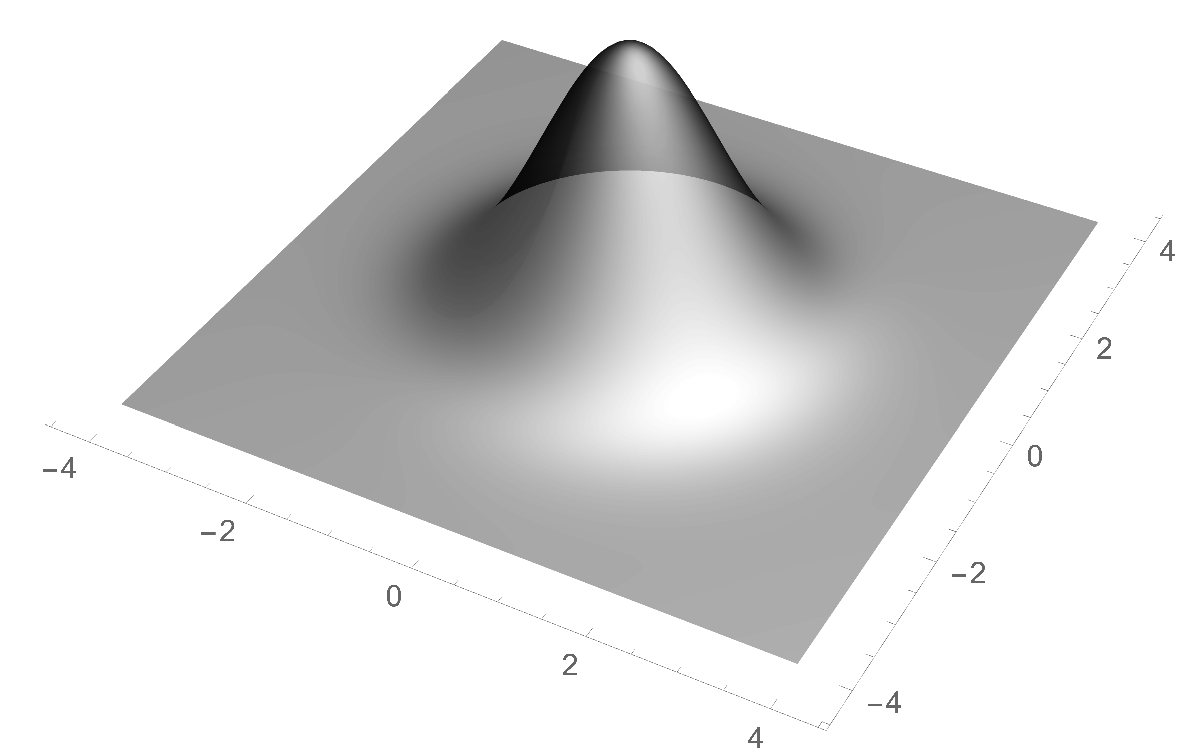
\includegraphics[scale=.3]{figures/hist-1.pdf}
  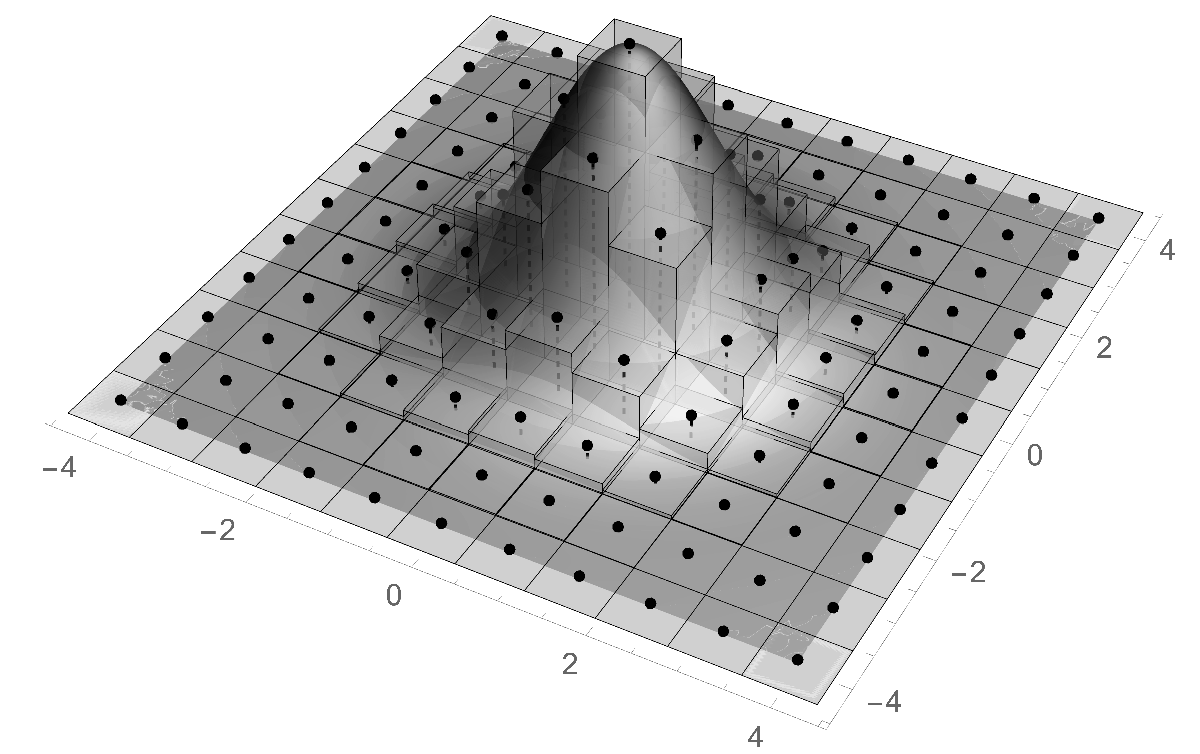
\includegraphics[scale=.3]{figures/hist-2.pdf} \\
  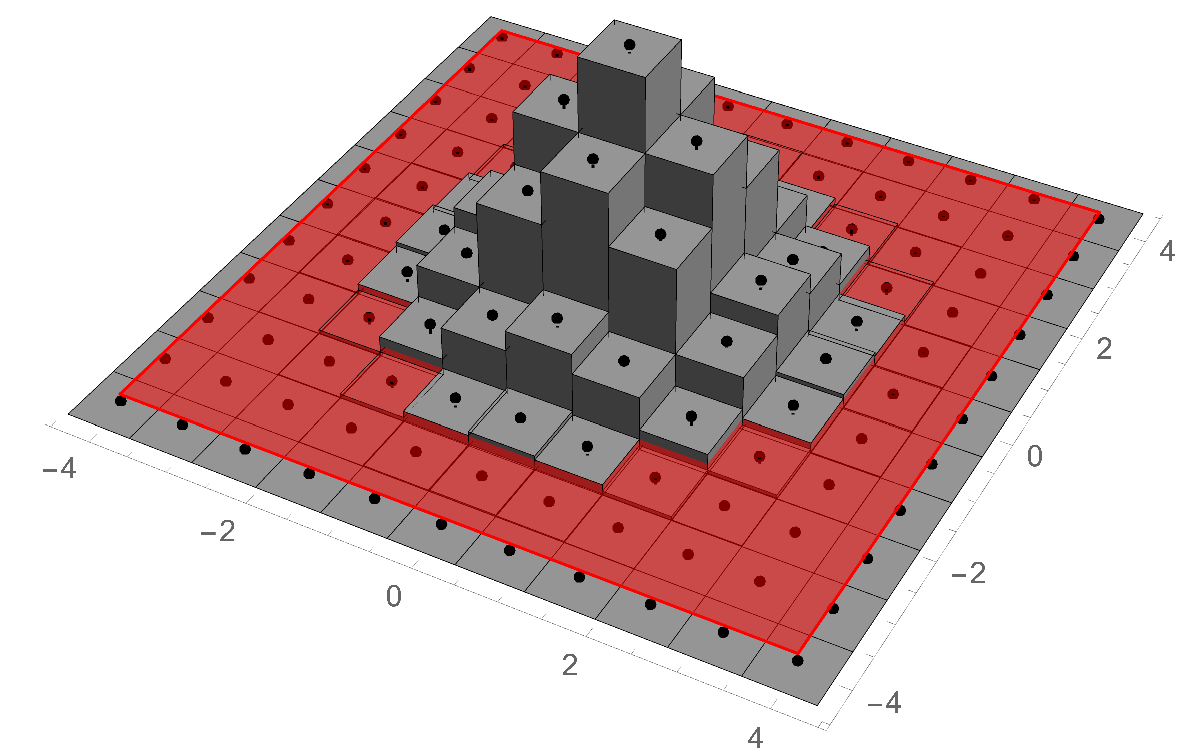
\includegraphics[scale=.3]{figures/hist-3.pdf}
  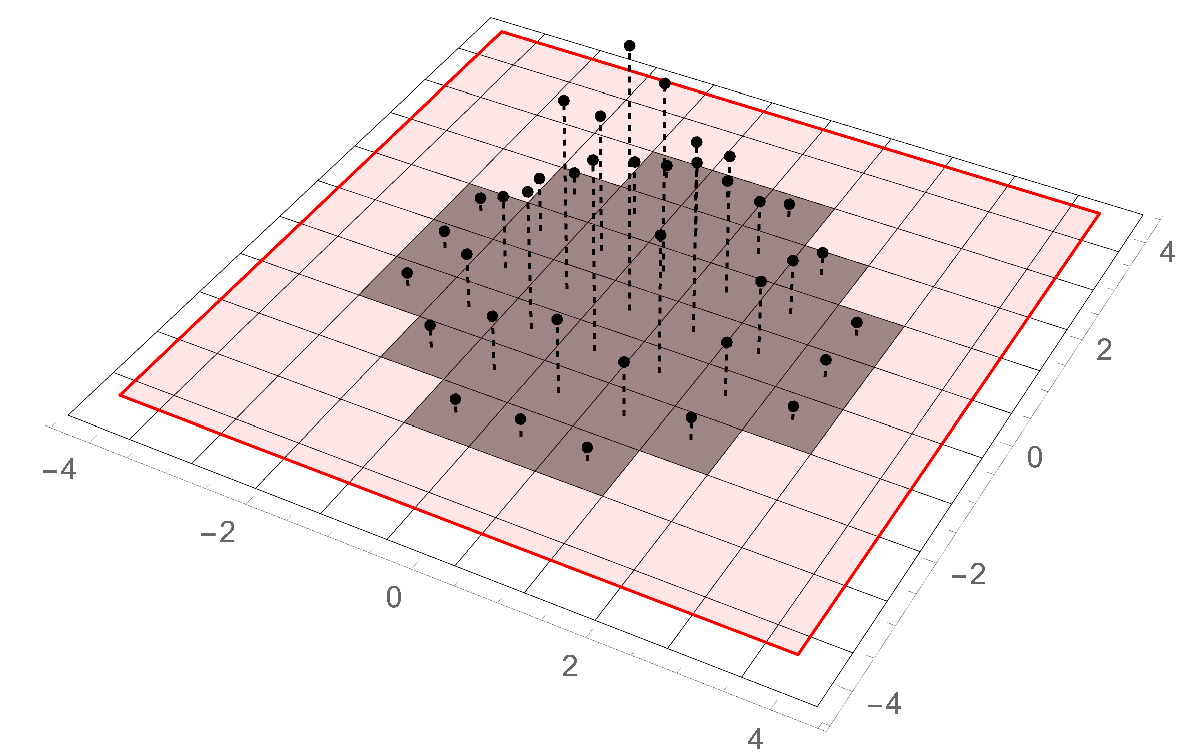
\includegraphics[scale=.3]{figures/hist-4.pdf} \\
  \caption{In two dimensions and by analogy with Figure~\ref{fig:hdr-1d-1}, $f_{\al}$ is computed by discretizing the density $f(x,y)$, and HDRs are constructed from points $(x_{i},y_{j})$ where $f(x_{i},y_{j}) \geq f_{\al}$. Here $\al = .05$ was used.}%
  \label{fig:hdr-2d-1}
\end{figure}


\begin{knitrout}
\definecolor{shadecolor}{rgb}{1, 1, 1}\color{fgcolor}\begin{figure}[h!]

{\centering 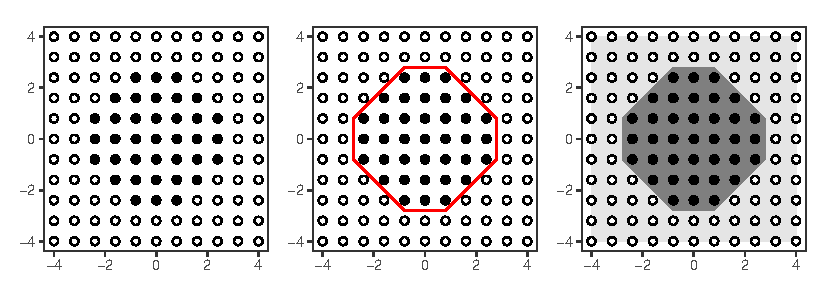
\includegraphics[width=\maxwidth]{figures/hdr-2d-2-1}

}

\caption{Figure~\ref{fig:hdr-2d-1} from the plane perspective. \CRANpkg{ggdensity} constructs HDRS by applying the marching squares contouring algorithm to binary grid where $f_{ij} \geq f_{\al}$ provided by \code{isolines()} and \code{isobands()}.}\label{fig:hdr-2d-2}
\end{figure}

\end{knitrout}


%
% \begin{figure}[h!]%
%   \centering
%   \includegraphics[width=9cm,height=3cm]{images/temp-3d-1.png}
%   \caption{Finding $\hat{f}_{.50}$ from a sample of bivariate normal data}%
%   \label{fig:3d-1}
% \end{figure}
%

\pagebreak

An alternative approach is worth mentioning at this point.
The method described above is essentially what \cite{hyndman_computing_1996} refers to as the ``numerical integration approach''.
However, alternative approaches exist.
\cite{hyndman_computing_1996} suggests using the simple, consistent quantile estimate $\hat{f}_{\al} = \hat{f}_{(j)}$, where $\hat{f}_{(j)}$ is the $\left(j/n\right)$ sample quantile of $\{ \hat{f}(x_i,y_i)\}$ and $j = \lfloor\alpha n\rfloor$.
Presented with data $(x_{1},y_{1}), \ldots, (x_{n}, y_{n})$, if $f(x,y)$ is known, any estimate of the $1-\al$ quantile of $f(X,Y)$ is an estimate of $f_{\al}$; this is referred to as the ``density quantile approach''.
Notice that this requires contours intersect at least one data point and forces a certain proportion of observed values outside of the HDRs, regardless of sample size.
Unavailable in \CRANpkg{ggdensity}, this method\footnote{There are many valid choices of $\hat{f}_{\al}$, \CRANpkg{hdrcde} and \CRANpkg{gghdr} make use of \code{stats::quantile()} with \code{type = 7} which estimates a continuous sample quantile function with linear interpolation, a slight modification of the strategy outlined in \cite{hyndman_computing_1996}.} is implemented in both \CRANpkg{hdrcde} \citep{hyndman_hdrcde_2021} and \CRANpkg{gghdr} \citep{ohara-wild_gghdr_2022}.



\newpage

%%%%%
%%%%%%%%%%%%%%%%%%%%%%%%%%%%%%%%%%%%%%%%%%%%%%%%%%%%%%%%%%%%
\subsection{HDRs using different density estimators}\label{sec:hdr-methods}

As we noted previously, sample HDRs can be computed using many density estimation methods.
Figure~\ref{fig:hdr-2d-est} illustrates how 95\% HDRs are calculated for histogram estimators and KDEs on a sample of size $n=1,000$ from the standard bivariate normal distribution.
These use the exact same method as previously described.




\begin{widefigure}[h!]%
  \centering
  % 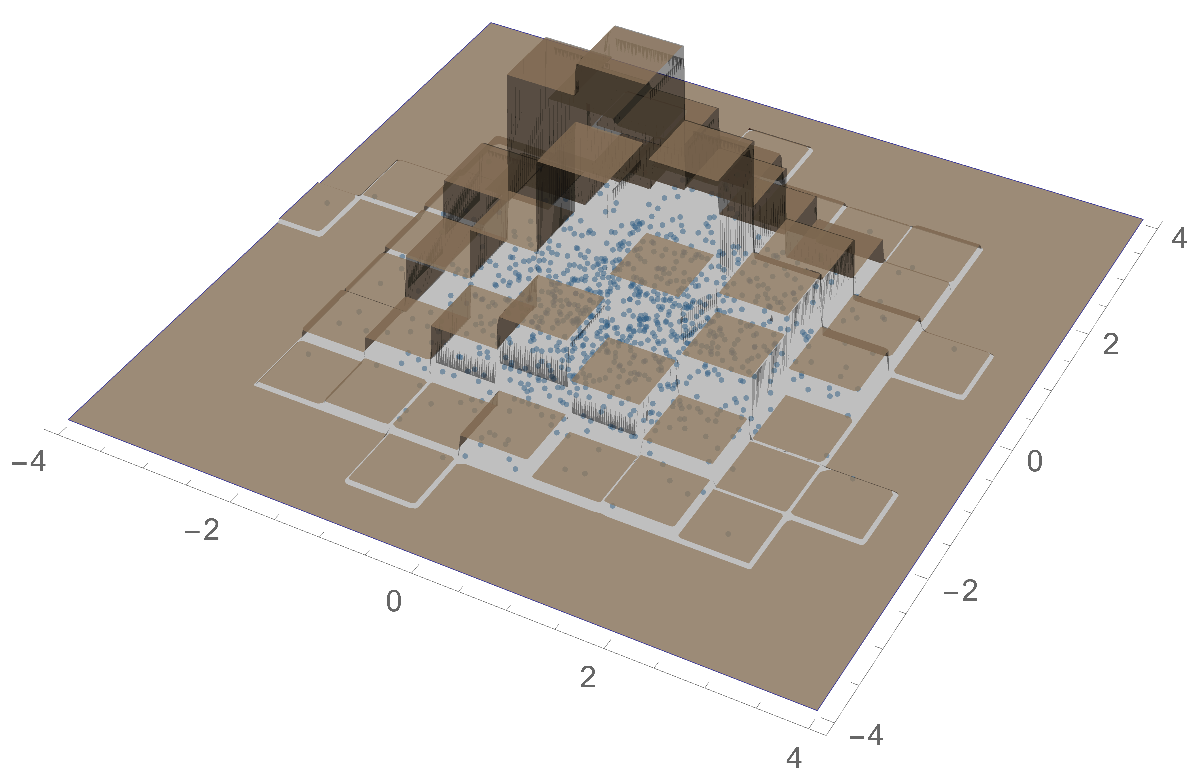
\includegraphics[scale=.275]{figures/fhat-hist-1.pdf}
  % 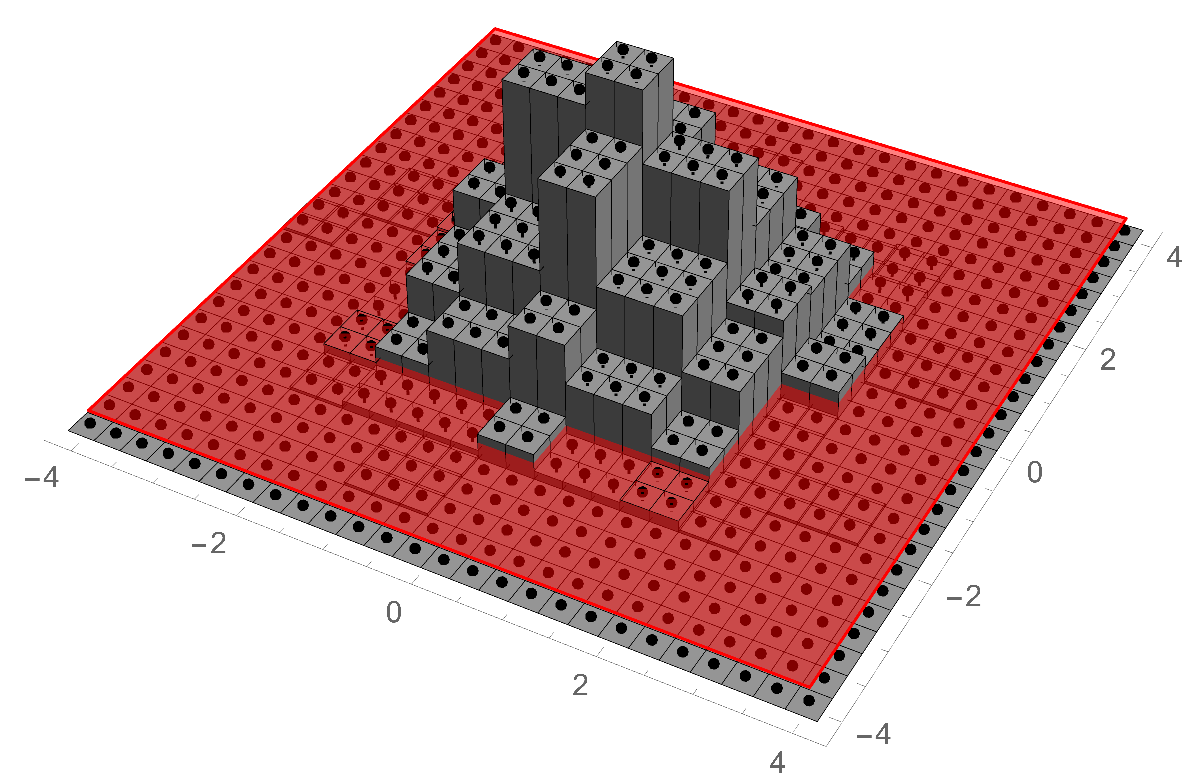
\includegraphics[scale=.275]{figures/fhat-hist-3.pdf}
  % 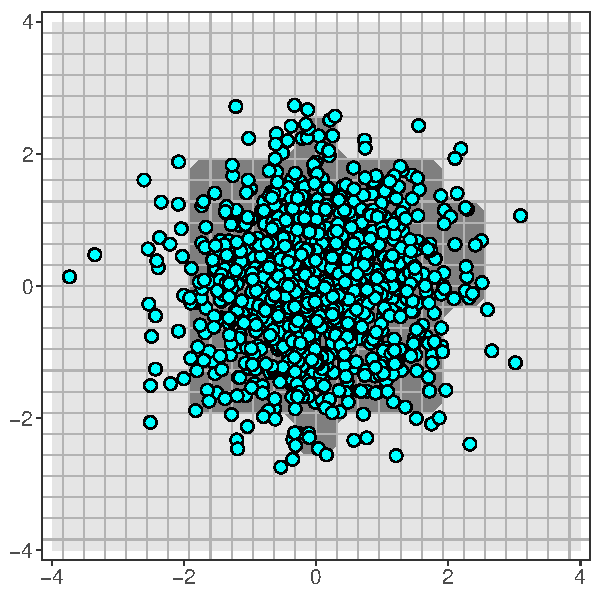
\includegraphics[scale=.425]{figures/fhat-hist-5.pdf} \\
  % 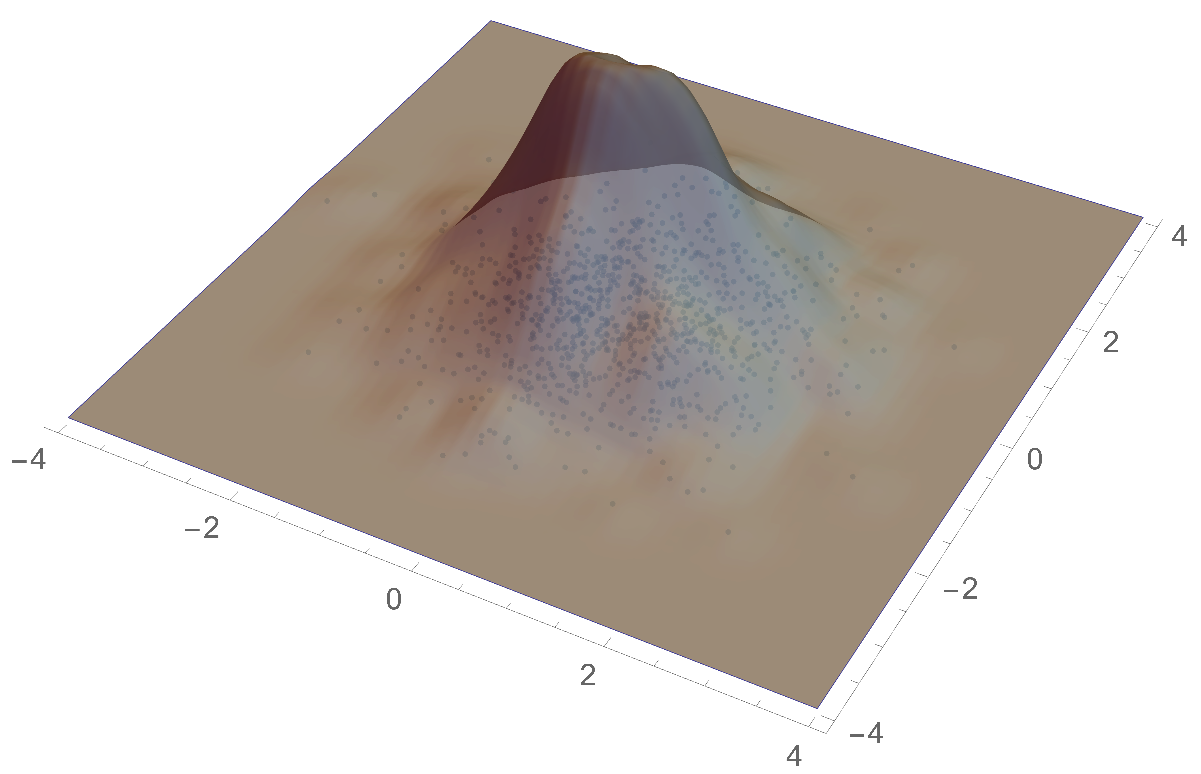
\includegraphics[scale=.275]{figures/fhat-kde-1.pdf}
  % 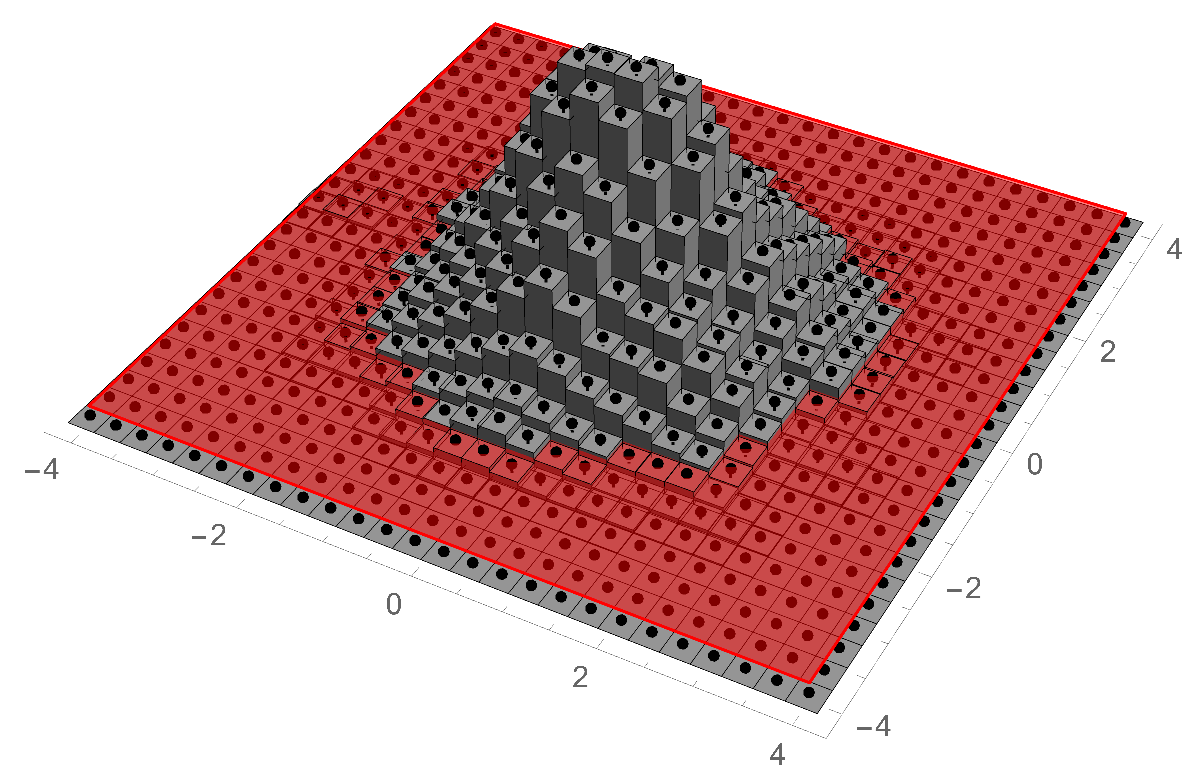
\includegraphics[scale=.275]{figures/fhat-kde-3.pdf}
  % 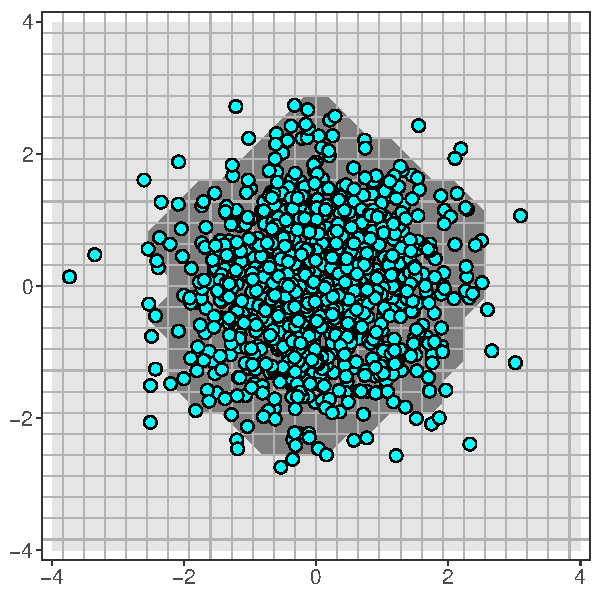
\includegraphics[scale=.425]{figures/fhat-kde-5.pdf}
  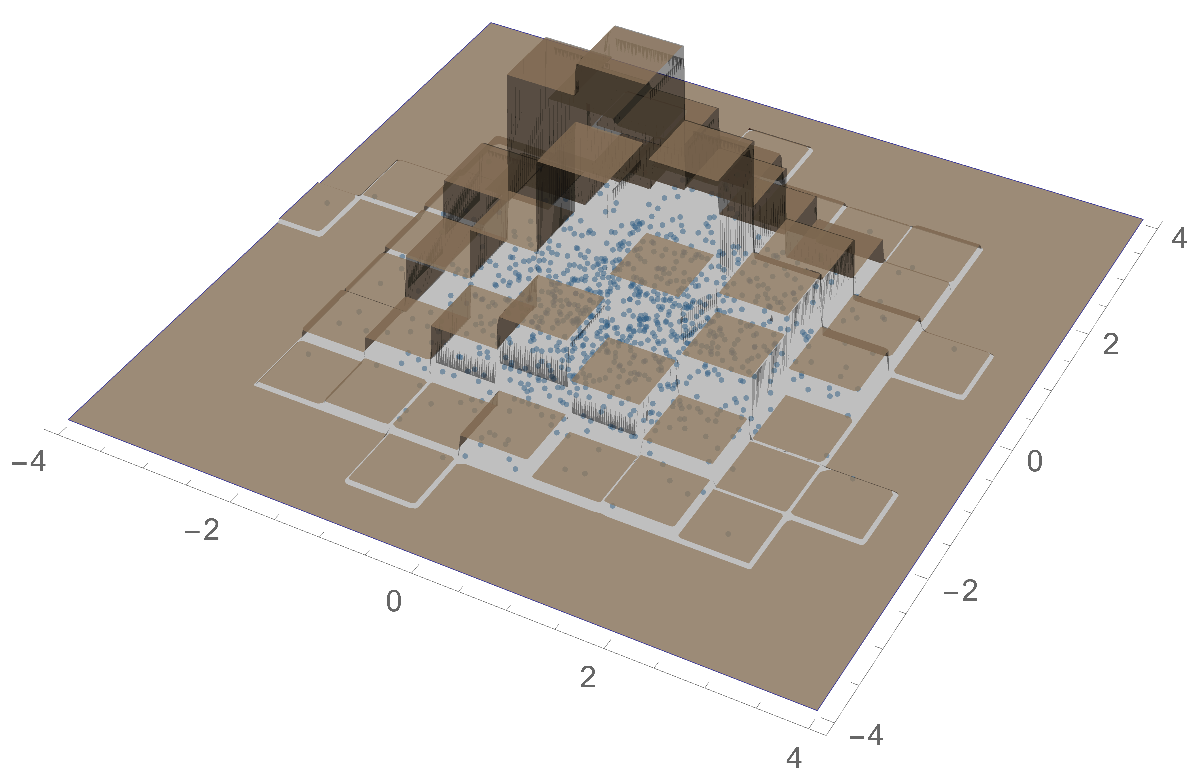
\includegraphics[scale=.225]{figures/fhat-hist-1.pdf}
  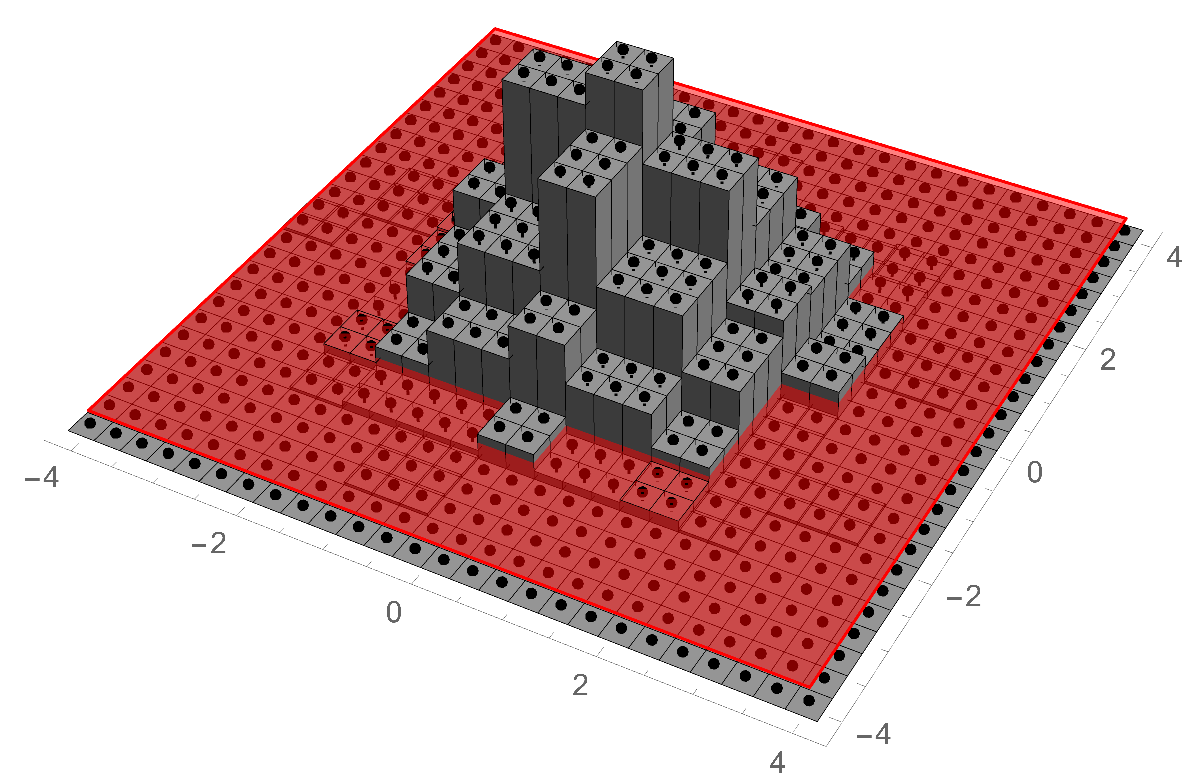
\includegraphics[scale=.225]{figures/fhat-hist-3.pdf}
  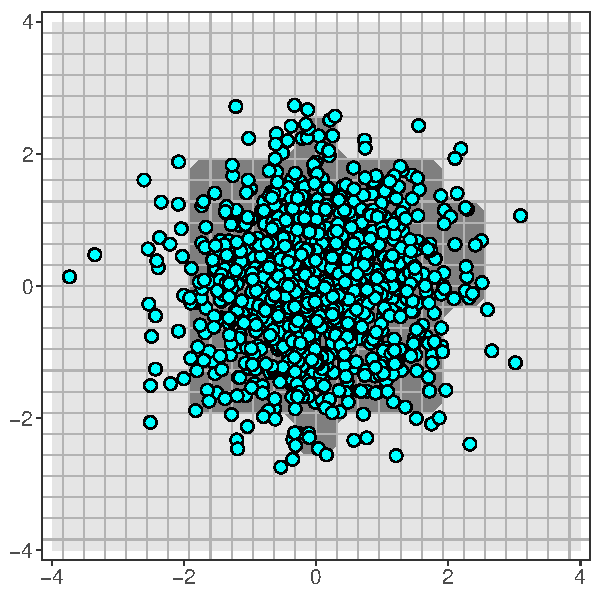
\includegraphics[scale=.357]{figures/fhat-hist-5.pdf} \\
  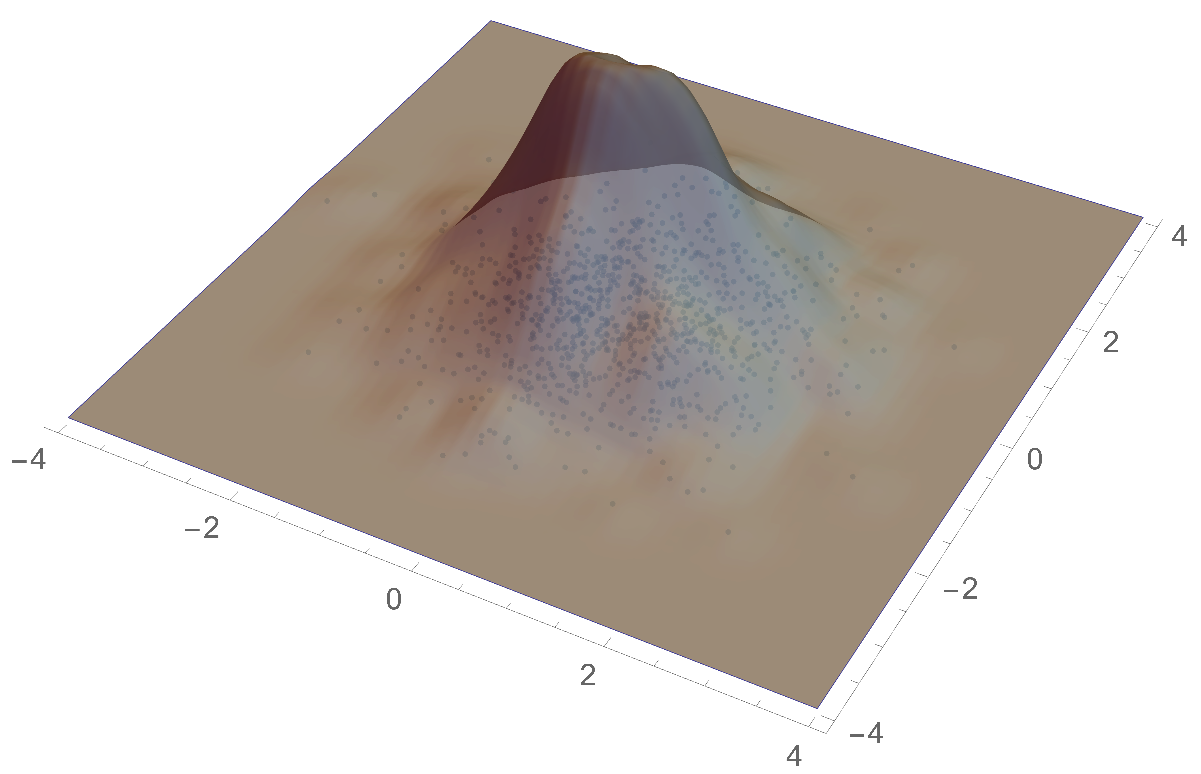
\includegraphics[scale=.225]{figures/fhat-kde-1.pdf}
  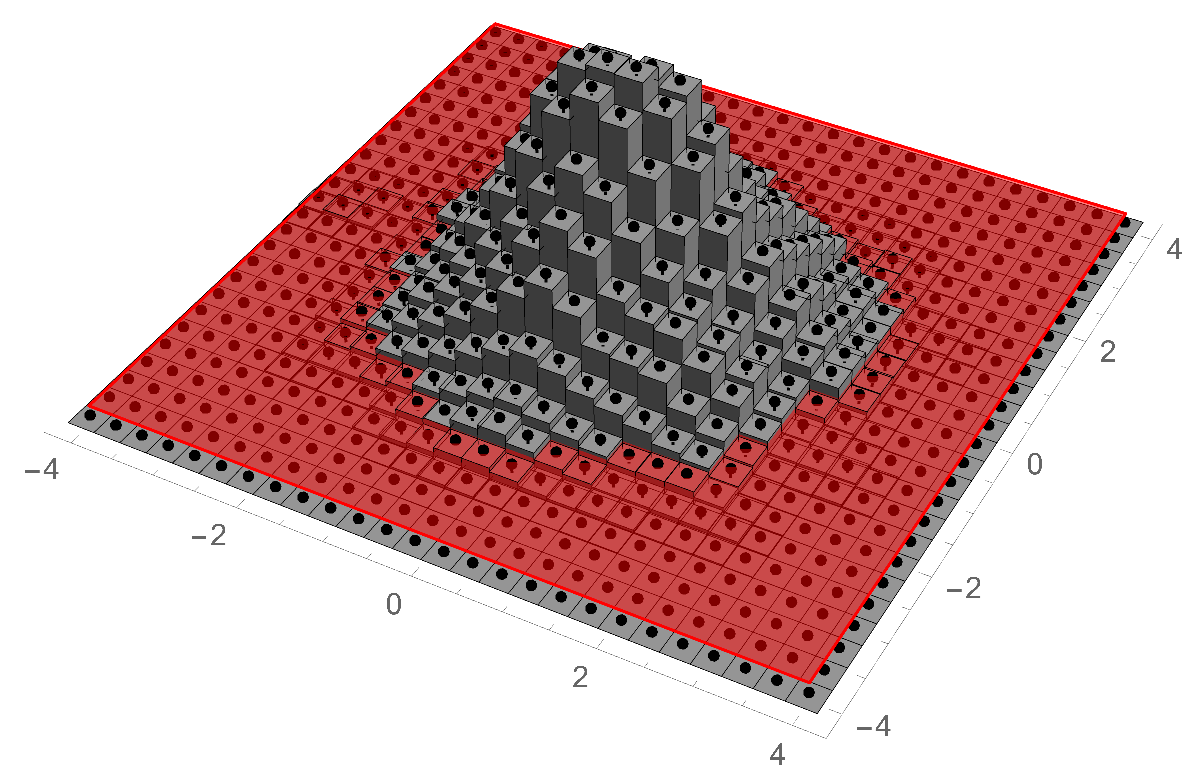
\includegraphics[scale=.225]{figures/fhat-kde-3.pdf}
  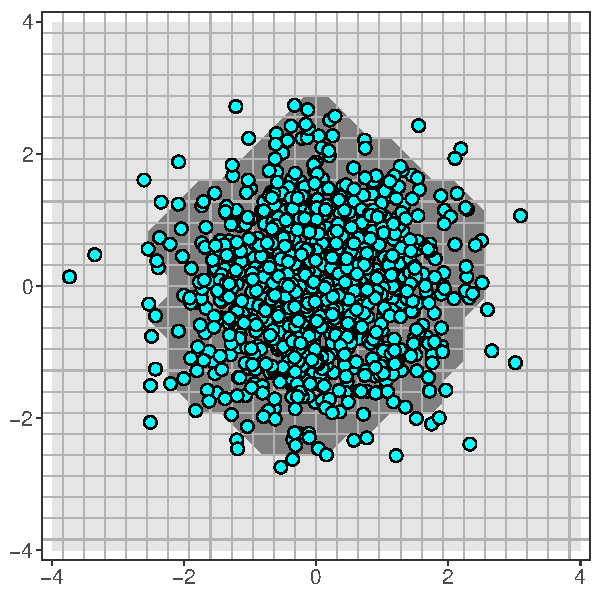
\includegraphics[scale=.357]{figures/fhat-kde-5.pdf}
  \caption{\CRANpkg{ggdensity} facilitates using different density estimators to determine HDRs, including histograms (top, 11 bins in each dimension) and kernel density estimators (bottom), the default. Here 95\% HDRs are illustrated using $N = 25$ and $n = 1,000$ draws from the standard bivariate normal distribution. The illustration refects the method of construction, not output of \code{geom\_hdr()}.}%
  \label{fig:hdr-2d-est}
\end{widefigure}


Figure~\ref{fig:ex-methods} displays the output of \code{geom\_hdr()} using the full range of methods available for three different simulated data sets with different features.
By default, \code{geom\_hdr()} and \code{geom\_hdr\_lines()} plot the 50\%, 80\%, 90\% and 95\% HDRs.
The methods are available in both \code{geom\_hdr()} and \code{geom\_hdr\_lines()} through the \code{method} argument, which allows for the specification of various nonparametric and parametric estimators, each offering advantages in certain contexts.
For example, histogram estimators result in HDRs that obey constrained supports.
Normal estimators, i.e. the best-fit bivariate normal estimator, can be helpful in providing simplified visuals that give the viewer a sense of where the distributions are, potentially at the expense of over-simplifying and removing important features of how the variables co-vary.









% These knitr options are super finicky
% Don't understand why, but we need to specify out.width/height + fig.asp
\begin{knitrout}
\definecolor{shadecolor}{rgb}{1, 1, 1}\color{fgcolor}\begin{widefigure}[p]

% {\centering 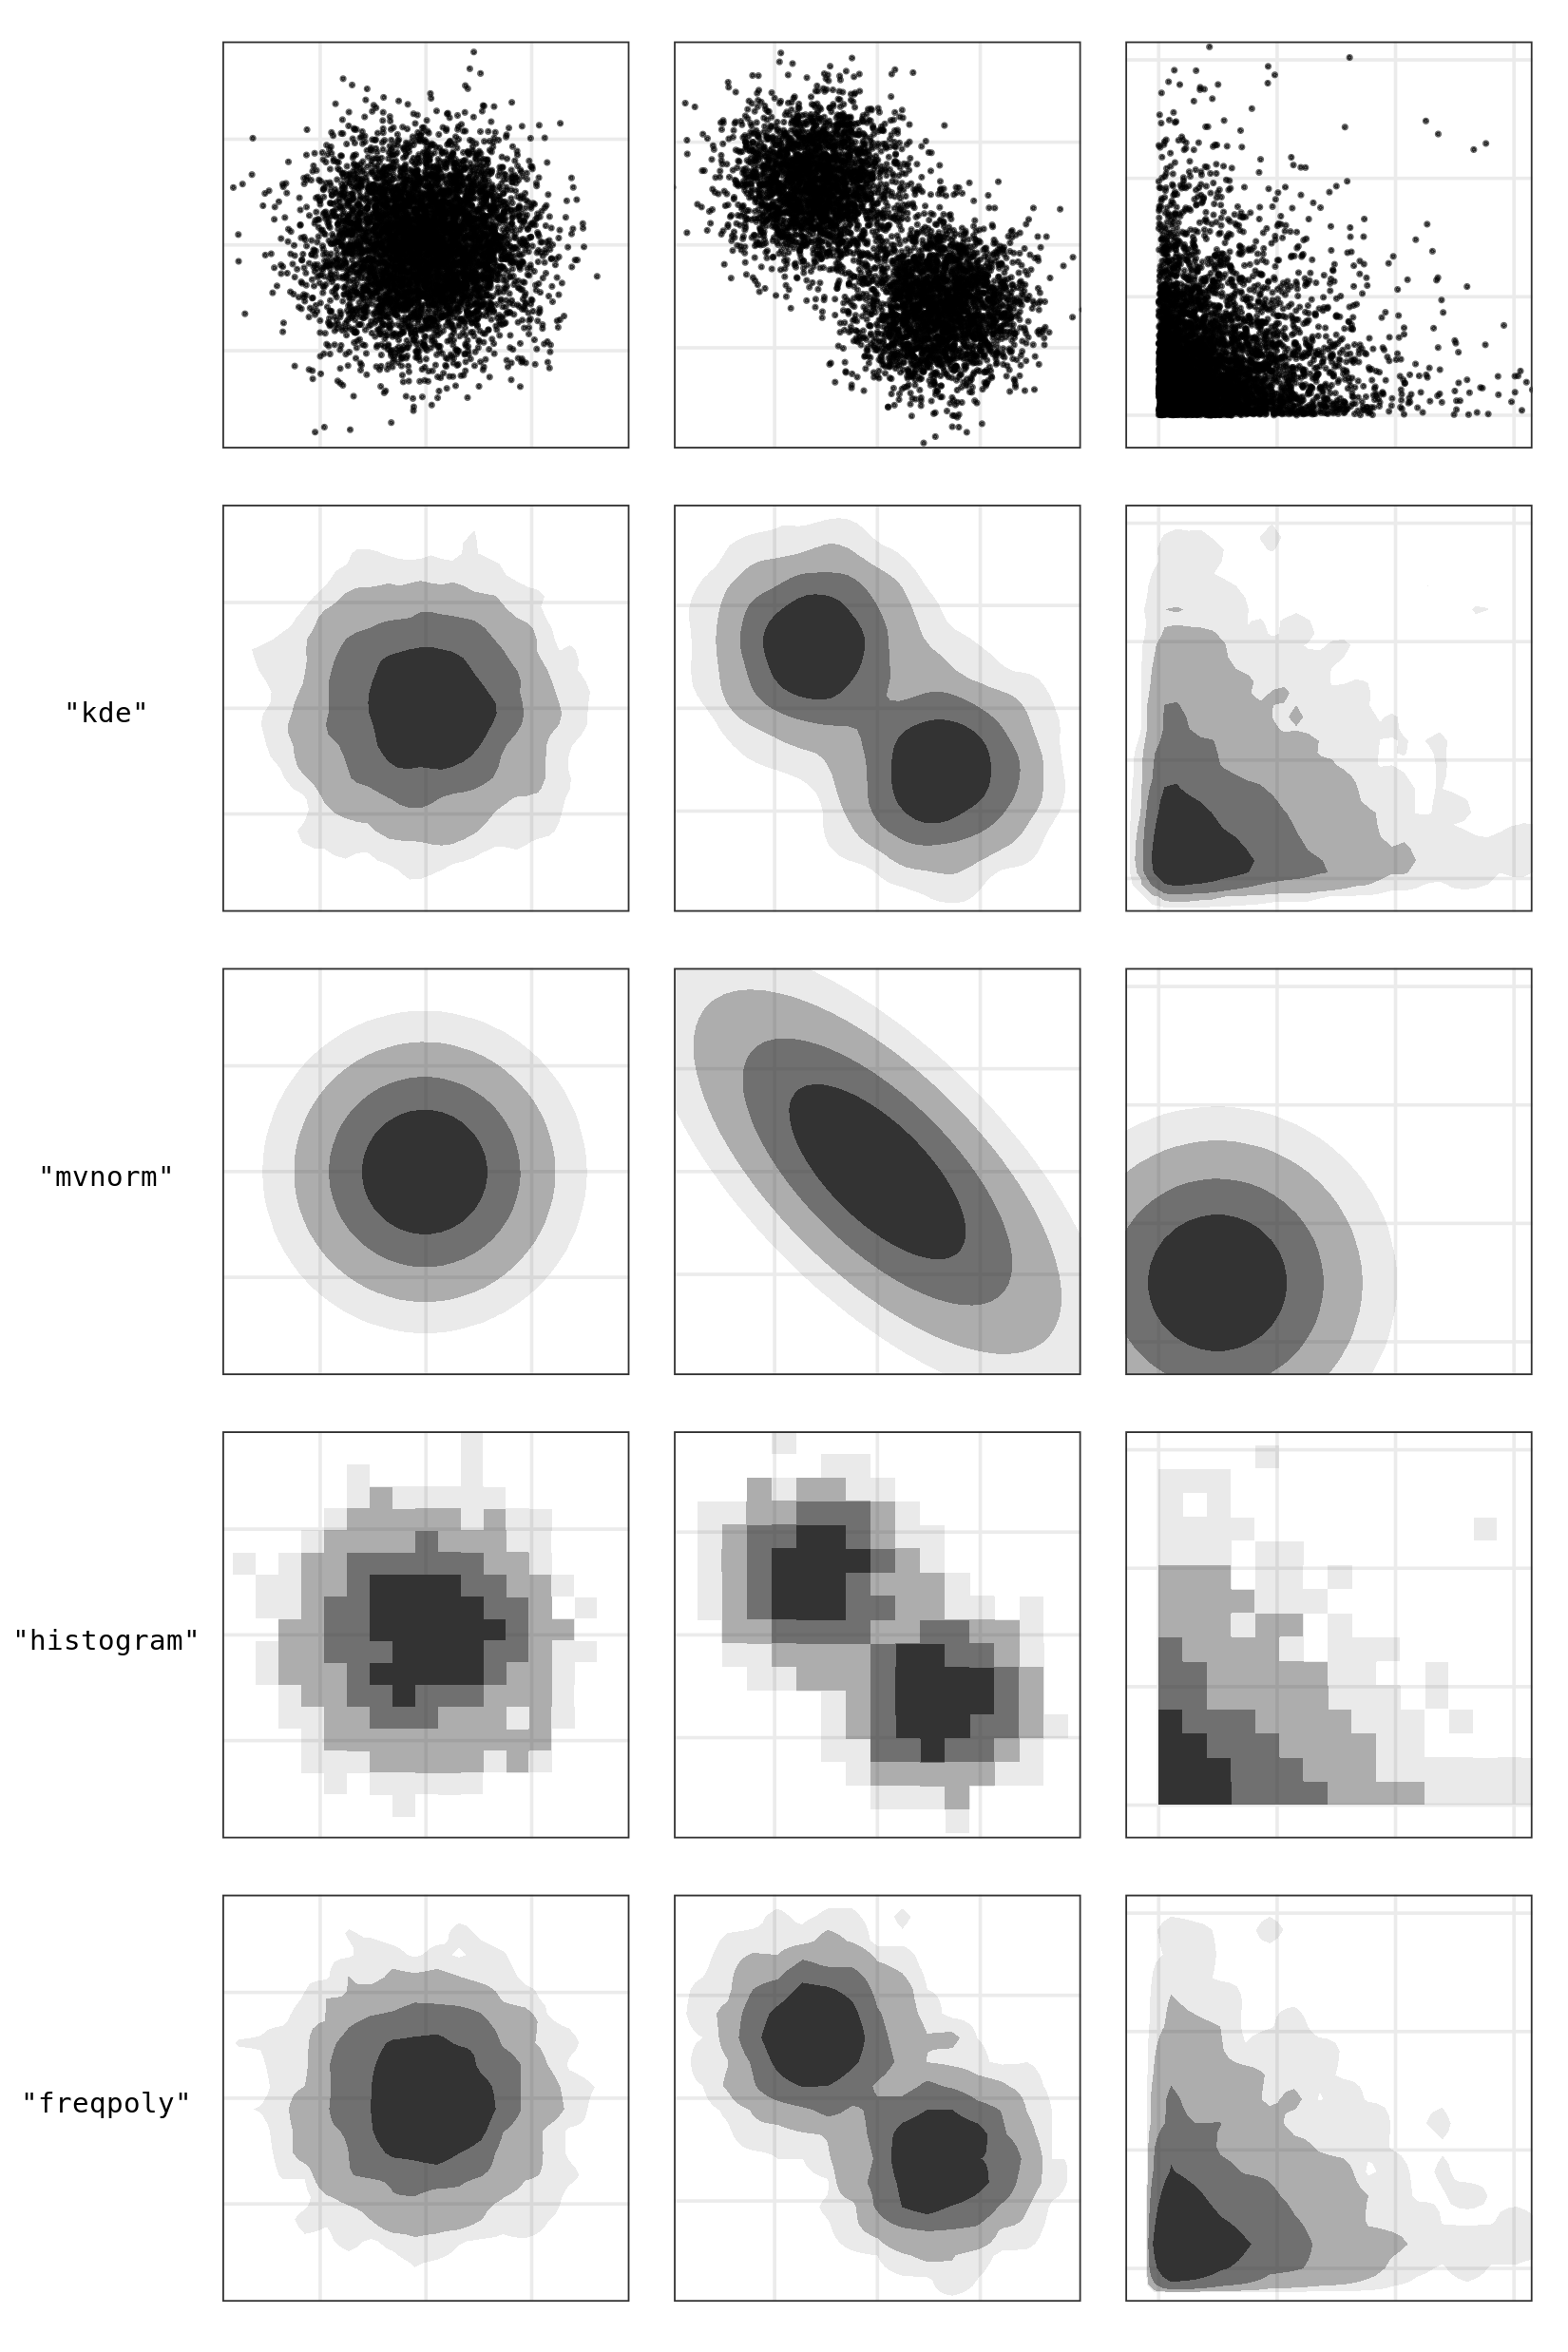
\includegraphics[width=6.5in,height=9.5in]{figures/ex-methods-1}
{\centering 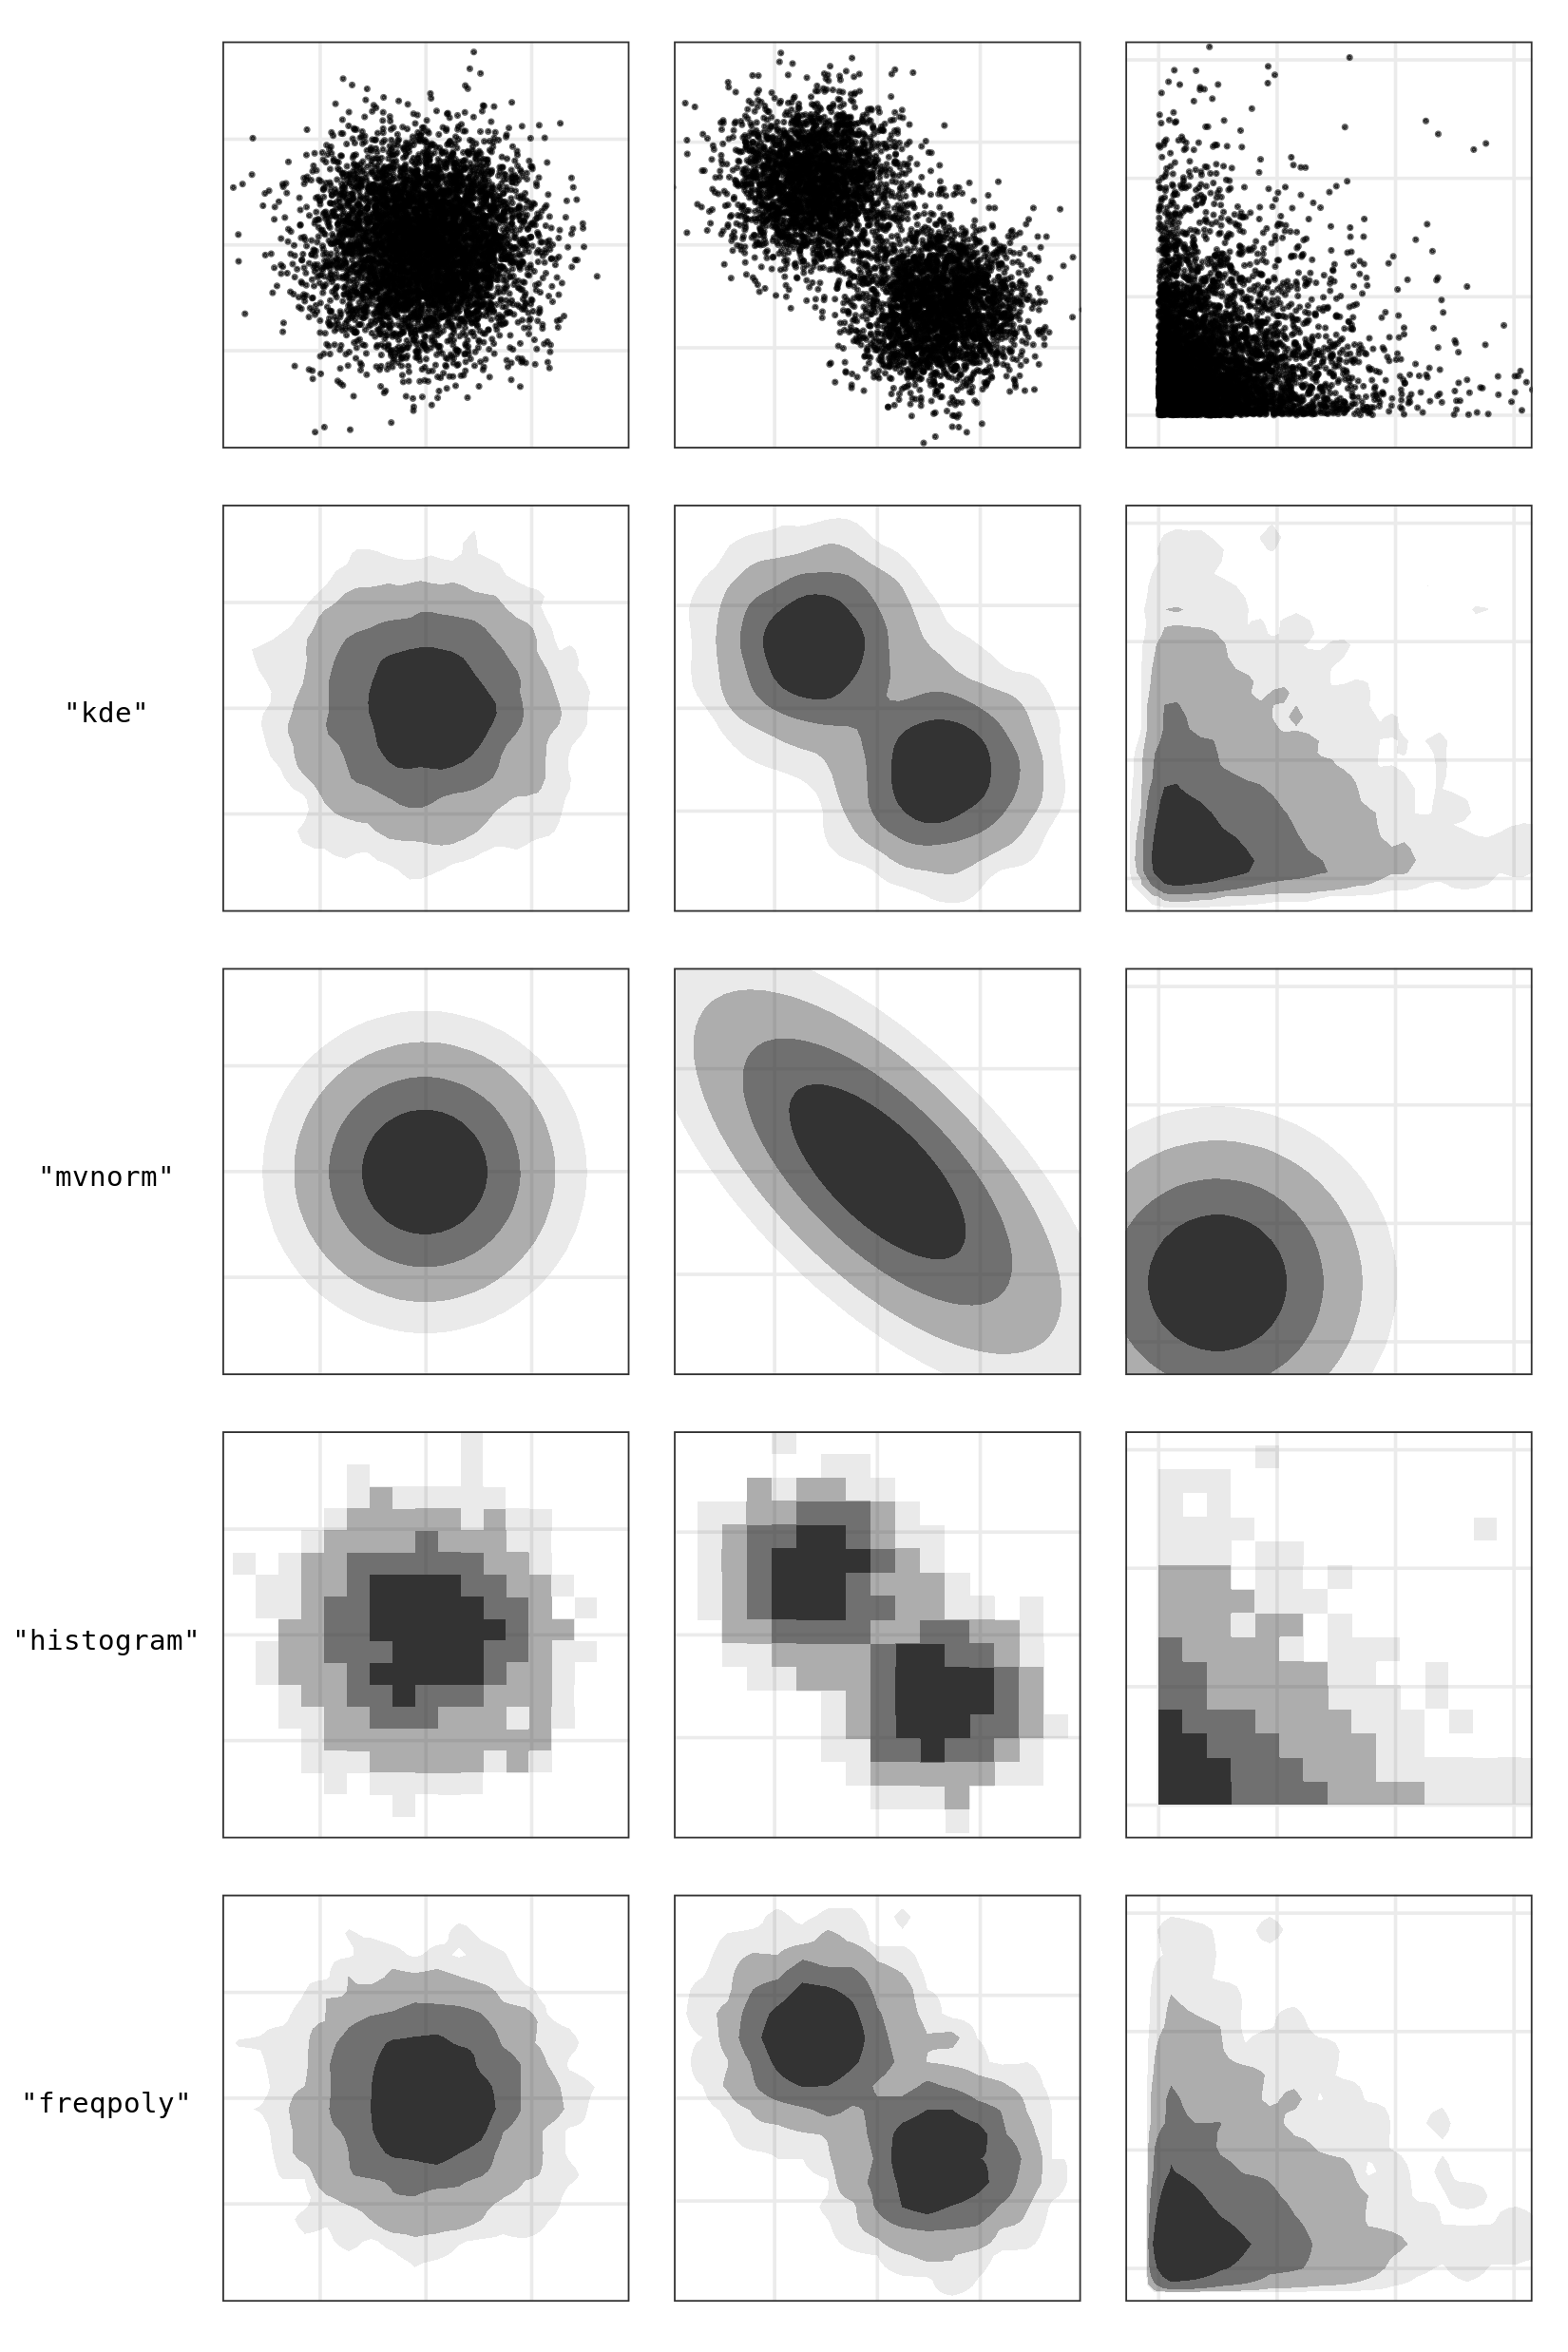
\includegraphics[width=5.5in,height=8in]{figures/ex-methods-1}

}

\caption{Comparing HDRs obtained with different {\tt method} arguments to \code{geom\_hdr()}.}\label{fig:ex-methods}
\end{widefigure}

\end{knitrout}




% 'Mapping to the fill aesthetic to plot multiple groups in the \\texttt{penguins} dataset, specifying \\texttt{method = "mvnorm"}'


\pagebreak
%%%%%
%%%%%%%%%%%%%%%%%%%%%%%%%%%%%%%%%%%%%%%%%%%%%%%%%%%%%%%%%%%%
\subsection{HDRs from known density functions}\label{sec:hdr-known}


The same method can be used to determine the HDRs of a given density function.
This is implemented for bivariate densities in \CRANpkg{ggdensity} as \code{geom\_hdr\_fun()} and \code{geom\_hdr\_lines\_fun()}, both accepting a PDF via the \code{fun} argument.
Figure~\ref{fig:eval-hdr-2d-known} illustrates this by plotting the HDRs of bivariate random vector $\mathbf{X} = (X_1, \; X_2)$ with $X_1 \perp X_2$, $X_1 \sim \mc{N}(0, 1)$ and $X_2 \sim \mathrm{Gamma}(5, 3)$ (left),
and $ \mathbf{Y} \sim f_{\mathbf{Y}}(y_1, y_2) \propto \exp \left\{ -\frac{1}{2 (.20)^2} (y_1^2 + y_2^2 - 1)^2 \right\}$ (right), which concentrates its probability along the unit circle $\mc{S}^1$.
In this case we make use of the fact that \code{geom\_hdr\_fun()} can find the HDRs of unnormalized PDFs.
It does so by leveraging the fact that over a given window, the discretization is not affected by whether or not the density is normalized.

\begin{knitrout}
\definecolor{shadecolor}{rgb}{1, 1, 1}\color{fgcolor}\begin{kframe}
\begin{example}
f_X <- function(x1, x2) dnorm(x1) * dgamma(x2, 5, 3)
ggplot() + geom_hdr_fun(fun = f_X, xlim = c(-4, 4), ylim = c(0, 5))
\end{example}
\end{kframe}
\end{knitrout}
\begin{knitrout}
\definecolor{shadecolor}{rgb}{1, 1, 1}\color{fgcolor}\begin{kframe}
\begin{example}
f_Y <- function(y1, y2) exp(-1/(2 * .20^2) * (y1^2 + y2^2 - 1)^2)
ggplot() +
  geom_hdr_fun(fun = f_Y, normalized = FALSE, xlim = c(-4, 4), ylim = c(-4, 4)) +
  coord_equal()
\end{example}
\end{kframe}
\end{knitrout}

\begin{knitrout}
\definecolor{shadecolor}{rgb}{1, 1, 1}\color{fgcolor}\begin{figure}[h!]

{\centering 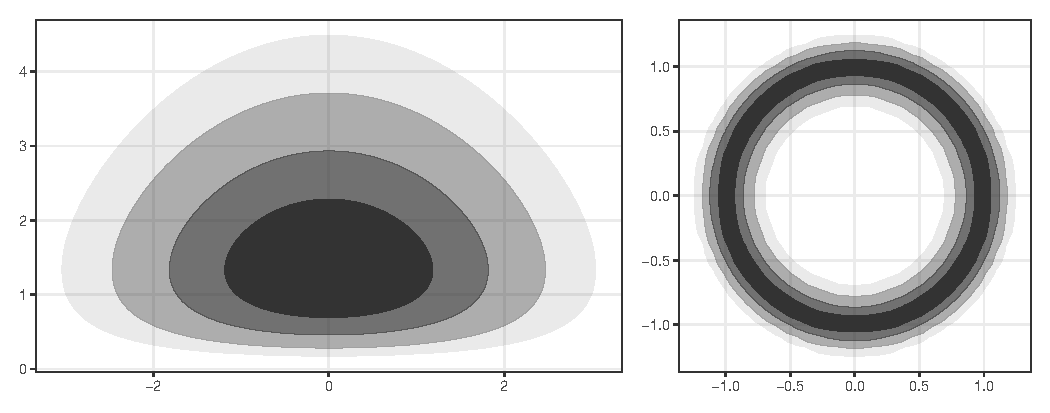
\includegraphics[width=\maxwidth]{figures/eval-hdr-2d-known-1}

}

\caption{\code{geom\_hdr\_fun()} can be used to plot HDRs of normalized and un-normalized known PDFs.}\label{fig:eval-hdr-2d-known}
\end{figure}

\end{knitrout}

In both of these examples, determining the exact contours is a nontrivial proposition.
However, we have not had to derive any results regarding the distributions of $\mathbf{X}$ or $\mathbf{Y}$ to plot them or find the values of $f_{\alpha}$ -- this is all been numerically approximated by \CRANpkg{ggdensity} via the previously discussed ``numerical integration'' method.
This represents a simple, powerful tool for visualizing and understanding the probabilistic behavior of arbitrary densities, so long as their support is roughly known.

Beyond the utility of visualizing HDRs of theoretical densities, \code{geom\_hdr\_fun()} and \code{geom\_hdr\_lines\_fun()} can be used to plot HDRs for arbitrary parametric estimates of $f$.
We discuss this at the end of the following section.


\pagebreak

%%%%%
%%%%%%%%%%%%%%%%%%%%%%%%%%%%%%%%%%%%%%%%%%%%%%%%%%%%%%%%%%%%%%%%%%%%%%%%%%%%%%%%
\section{Further examples}\label{sec:further-examples}

We conclude with a series of more advanced examples that illustrate the flexibility and power of \CRANpkg{ggdensity} through more complicated use-cases.


%%%%%
%%%%%%%%%%%%%%%%%%%%%%%%%%%%%%%%%%%%%%%%%%%%%%%%%%%%%%%%%%%%
\subsection{Comparing populations}\label{sec:populations}


Since \code{geom\_hdr()} and \code{geom\_hdr\_lines()} use transparency (the \code{alpha} aesthetic) to communicate probability,
color remains available to communicate group membership in the context of more than one population via either the \code{fill} or \code{color} aesthetics.
This allows for easy comparison of multiple bivariate populations via their HDRs.
In Figure~\ref{fig:palmer_penguins}, we use this strategy to compare the relationship between flipper length and bill length for different species of penguins using the popular Palmer penguins dataset \citep{horst_palmerpenguins_2020}.
In this case \code{geom\_hdr\_lines()} is used to reduce overplotting.

As discussed previously, \CRANpkg{ggdensity} provides several nonparametric and parametric estimators to compute the HDRs.
Figure~\ref{fig:palmer_penguins} assumes a bivariate normal distribution, expressed by setting \code{method = "mvnorm"} in \code{geom\_hdr\_lines()}.
This implies that each group's HDRs are elliptical and the resulting visualization is a useful
approximation of the true distributions.
With it we can easily see the general location of each of the groups and that all have similar covariance structures.
These details can be obscured when more flexible non-parametric HDR estimators are used, especially when sample sizes are small.

% In addition to the kernel density and bivariate normal methods, \code{geom\_hdr()} and \code{geom\_hdr\_lines()} also implement histogram and frequency polygon HDR estimators.

\begin{knitrout}
\definecolor{shadecolor}{rgb}{1, 1, 1}\color{fgcolor}\begin{kframe}
\begin{example}
ggplot(penguins, aes(flipper_length_mm, bill_length_mm, fill = species)) +
  geom_hdr_lines(aes(color = species), method = "mvnorm") +
  geom_jitter(shape = 21)
\end{example}
\end{kframe}
\end{knitrout}
\begin{knitrout}
\definecolor{shadecolor}{rgb}{1, 1, 1}\color{fgcolor}\begin{figure}[h!]

{\centering 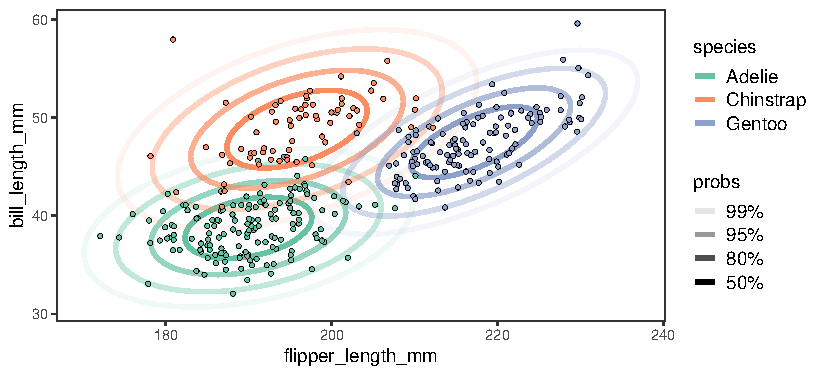
\includegraphics[width=\maxwidth]{figures/palmer_penguins-1}

}

\caption{Using \code{geom\_hdr\_lines()} with a color aesthetic can be used to reduce overplotting when visualizing the HDRs for different subgroups of data.}\label{fig:palmer_penguins}
\end{figure}

\end{knitrout}


%%%%%
%%%%%%%%%%%%%%%%%%%%%%%%%%%%%%%%%%%%%%%%%%%%%%%%%%%%%%%%%%%%
\subsection{HDRs and goodness of fit}\label{sec:hdr-gof}

It can be useful to combine \code{geom\_hdr()} and \code{geom\_hdr\_lines()} to compare different estimators of $f$.
A powerful example is plotting elliptical contour lines corresponding to an estimated normal model on top of filled contours of the KDE, facilitating a visual exploration of goodness of fit.
We have included two examples of this strategy in Figure~\ref{fig:normality_create_vis}.
The left graphic illustrates bill length versus flipper length for the Chinstrap penguins from Figure~\ref{fig:palmer_penguins}.
Notice that the filled contours generally match the contour lines, providing visual evidence towards the validity of an assumption of normality.
By contrast, the right graphic explores the relationship between two measurements from a dataset comparing 178 wines from \cite{forina_multivariate_1986} exported as \code{wines} in \CRANpkg{sn} \citep{azzalini_sn_2022}.
The filled contours do not coincide with the contour lines -- the nonparametric estimate of the density is visibly more skewed -- indicating that a normal approximation might not be appropriate for this data.

\pagebreak

\begin{knitrout}
\definecolor{shadecolor}{rgb}{1, 1, 1}\color{fgcolor}\begin{kframe}
\begin{example}
penguins |>
  filter(species == "Chinstrap") |>
  ggplot(aes(flipper_length_mm, bill_length_mm)) +
  geom_hdr() +
  geom_hdr_lines(color = "red", method = "mvnorm") +
  geom_jitter(color = "red")
\end{example}
\end{kframe}
\end{knitrout}

\begin{knitrout}
\definecolor{shadecolor}{rgb}{1, 1, 1}\color{fgcolor}\begin{kframe}
\begin{example}
ggplot(wines, aes(uronic, malic)) +
  geom_hdr() +
  geom_hdr_lines(method = "mvnorm", color = "red") +
  geom_jitter(color = "red")
\end{example}
\end{kframe}
\end{knitrout}


\begin{knitrout}
\definecolor{shadecolor}{rgb}{1, 1, 1}\color{fgcolor}\begin{widefigure}[h!]

{\centering 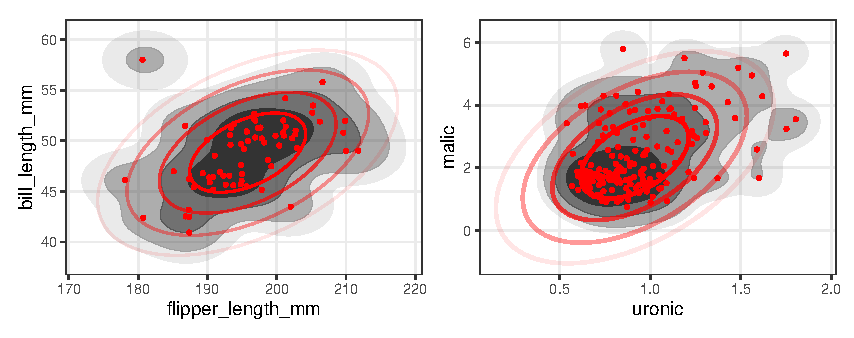
\includegraphics[width=\maxwidth]{figures/normality_create_vis-1}

}

\caption{Normality can be visually assessed by layering the HDRs of a KDE (black) with that of a parametrically estimated bivariate normal (red), here illustrated with Palmer penguin data (left) and wines data (right). The points in each plot have been jittered due to rounding in the data, notice that this leads to small inconsistencies between the plotted data and HDRs.}\label{fig:normality_create_vis}
\end{widefigure}

\end{knitrout}

This strategy can be extended to evaluating goodness of fit for arbitrary parametric models via combining \code{geom\_hdr()} and \code{geom\_hdr\_lines\_fun()},
following the strategy outlined in \nameref{hdr-fun}.



%%%%%
%%%%%%%%%%%%%%%%%%%%%%%%%%%%%%%%%%%%%%%%%%%%%%%%%%%%%%%%%%%%
\subsection{Other related geoms}\label{sec:other-geoms}

% \subsection{\code{geom\_hdr\_points()} and \code{geom\_hdr\_rug()}}
% \subsection{Other ways to visualize HDRs}

\CRANpkg{ggdensity} also includes functions \code{geom\_hdr\_points()} and \code{geom\_hdr\_rug()} for alternative methods of visualizing HDRs\footnote{
The previously mentioned \CRANpkg{gghdr} includes similar tools, we discuss this further in \nameref{sec:discussion}.
}.
These are illustrated in Figure~\ref{fig:eval_misc_vis}, in which we visualize the old faithful dataset \citep{azzalini_look_1990}.
The left image displays the standard visualization of HDRs from \code{geom\_hdr()}.
The graphic in the middle, created by \code{geom\_hdr\_points()}, displays the data itself with points colored by their HDR membership--this
can be useful in situations where overplotting is a concern.
The plot on the right presents the original data with the estimated marginal HDRs via \code{geom\_hdr\_rug()}.
Note that the scale is the same across all of the plots, with the 50\%, 80\%, 95\%, and 99\% HDRs being visualized by default.

\begin{knitrout}
\definecolor{shadecolor}{rgb}{1, 1, 1}\color{fgcolor}\begin{kframe}
\begin{example}
p <- ggplot(faithful, aes(eruptions, waiting))

p + geom_hdr()
p + geom_hdr_points()
p + geom_hdr_rug()
\end{example}
\end{kframe}
\end{knitrout}

\newpage

\begin{knitrout}
\definecolor{shadecolor}{rgb}{1, 1, 1}\color{fgcolor}\begin{widefigure}[h!]

{\centering 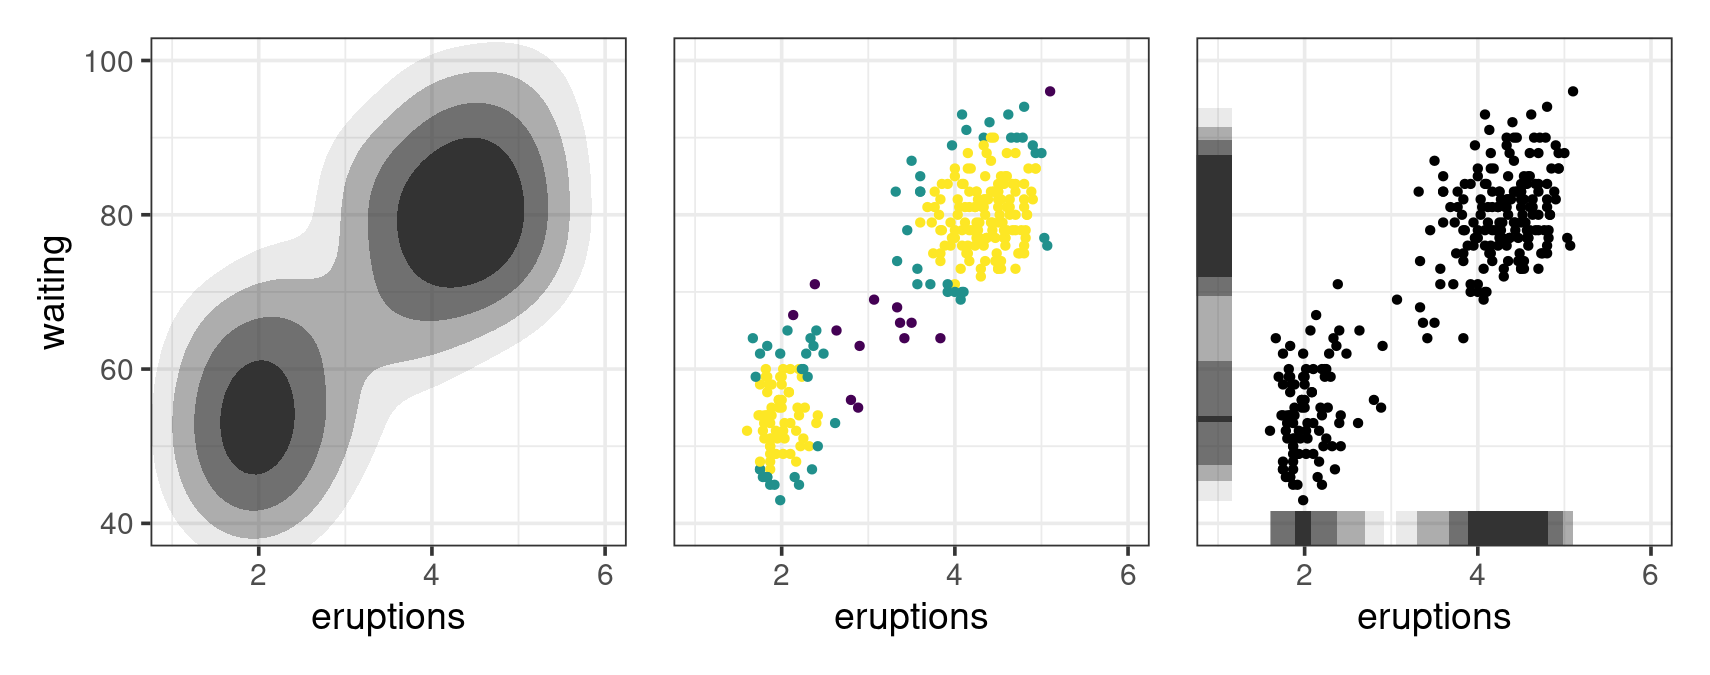
\includegraphics[width=\maxwidth]{figures/eval_misc_vis-1}

}

\caption{\code{geom\_hdr\_points()} and \code{geom\_hdr\_rug()} can provide more insight into bivariate scatterplots, as seen here with the faithful dataset.}\label{fig:eval_misc_vis}
\end{widefigure}

\end{knitrout}


It is important to note that \code{geom\_hdr\_rug()} can also be used when only an \code{x} or \code{y} aesthetic is provided.
This is illustrated in Figure~\ref{fig:eval_misc_vis_2} where the KDE of eruption duration is visualized alongside its estimated HDRs.
In this graphic we have chosen to communicate the HDRs via colors -- in some cases we have found this to be preferable when using \code{geom\_hdr\_rug()}.

\begin{knitrout}
\definecolor{shadecolor}{rgb}{1, 1, 1}\color{fgcolor}\begin{kframe}
\begin{example}
ggplot(faithful, aes(eruptions)) +
  geom_density() +
  geom_hdr_rug(aes(fill = after_stat(probs)), length = unit(.05, "npc"), alpha = 1) +
  scale_fill_viridis_d(option = "magma", begin = .8, end = 0)
\end{example}
\end{kframe}
\end{knitrout}

\begin{knitrout}
\definecolor{shadecolor}{rgb}{1, 1, 1}\color{fgcolor}\begin{widefigure}[h!]

{\centering 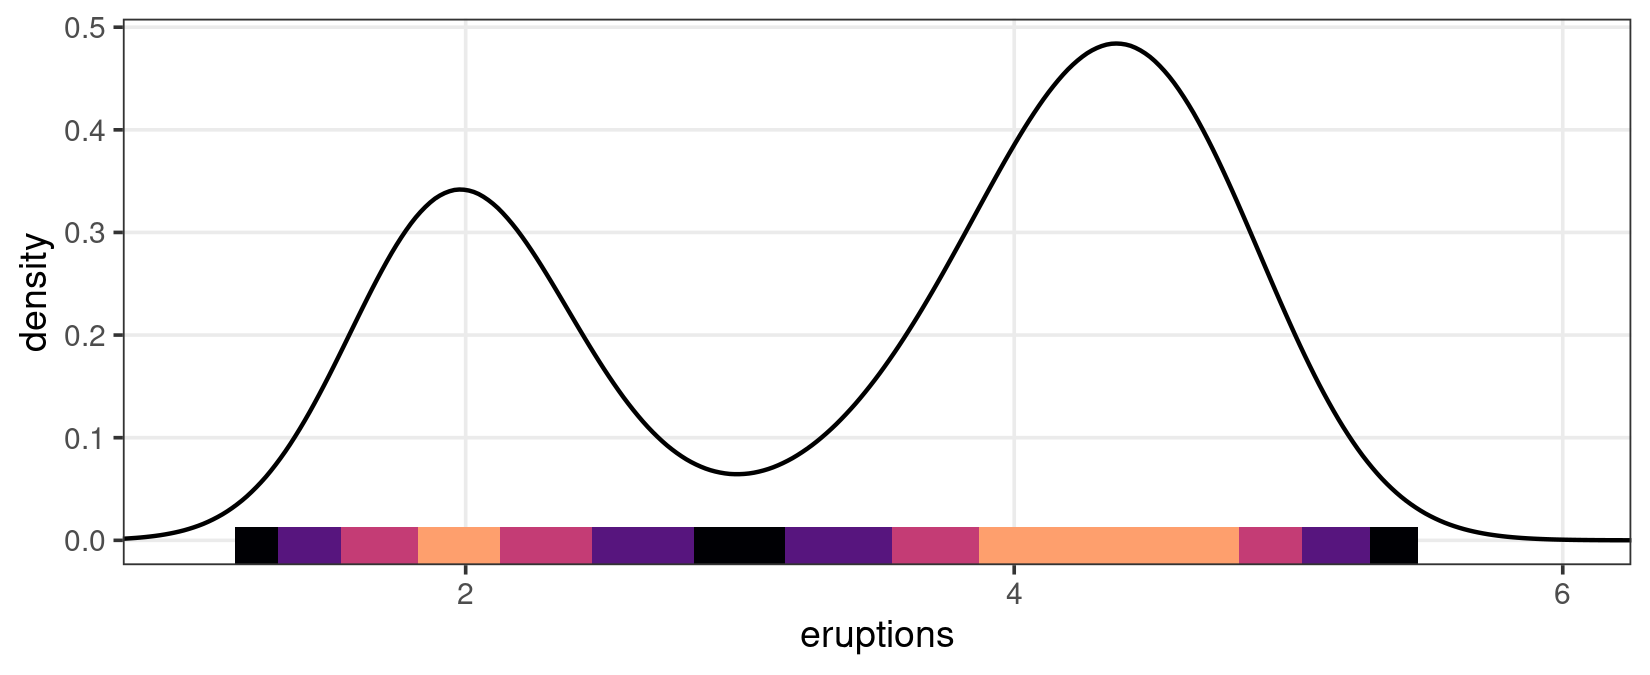
\includegraphics[width=\maxwidth]{figures/eval_misc_vis_2-1}

}

\caption{\code{geom\_hdr\_rug()} can also improve the visualization of univariate densities.}\label{fig:eval_misc_vis_2}
\end{widefigure}

\end{knitrout}











%%%%%
%%%%%%%%%%%%%%%%%%%%%%%%%%%%%%%%%%%%%%%%%%%%%%%%%%%%%%%%%%%%
\subsection{HDRs for arbitrary parametric models}\label{sec:parametric}
\label{hdr-fun}

% Difficult to say this, hard to know that DNE literature:
Historically, there has been much focus on contour estimation based on non-parametric estimates of $f$, typically KDEs.
To our knowledge, there has been relatively little focus on parametric estimation of HDRs.
If a probability model is specified, estimated HDRs are simple to derive from $\hat{f}_{\mathrm{MLE}}$, the density's maximum likelihood estimator (MLE).
This allows for the visualization of a much larger class of HDR estimators than those built into \code{geom\_hdr()};
users can specify and estimate arbitrary parametric models and provide the resulting density estimate to \code{geom\_hdr\_fun()}.

We include an example of HDRs corresponding to a custom estimated parametric density in Figure~\ref{fig:exp_example}.
Here we generated $n = 100$ draws from a bivariate exponential distribution $(X,Y) \sim f(x,y|\bm{\th}) = \mathrm{Exp}(\bm{\th})$,
estimated $\bm{\th}$ with its MLE, and passed the resulting estimate $\hat{f}(x,y) = f(x,y|\hat{\bm{\th}})$ to \code{geom\_hdr\_fun()} via the \code{fun} argument.

\begin{knitrout}
\definecolor{shadecolor}{rgb}{1, 1, 1}\color{fgcolor}\begin{kframe}
\begin{example}
set.seed(1)

df <- data.frame(x = rexp(100, 1), y = rexp(100, 1))

# pdf for parametric density estimate
f <- function(x, y, lambda) dexp(x, lambda[1]) * dexp(y, lambda[2])

# estimate parameters governing joint pdf
lambda_hat <- apply(df, 2, mean)

ggplot(df, aes(x, y)) +
  geom_hdr_fun(fun = f, args = list(lambda = lambda_hat)) +
  geom_point(fill = "lightgreen", shape = 21) +
  coord_fixed() +
  scale_x_continuous(limits = c(0, 7)) +
  scale_y_continuous(limits = c(0, 7))
\end{example}
\end{kframe}
\end{knitrout}
\begin{knitrout}
\definecolor{shadecolor}{rgb}{1, 1, 1}\color{fgcolor}\begin{widefigure}[h!]

{\centering 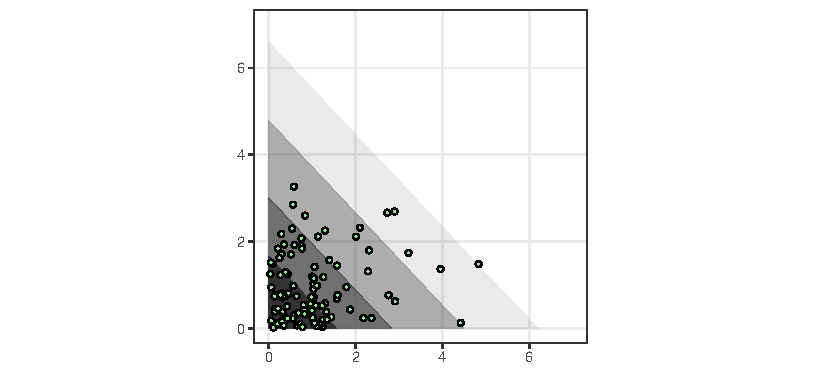
\includegraphics[width=\maxwidth]{figures/exp_example-1}

}

\caption{Plotting HDRs of specified distributions can be achieved with \code{geom\_hdr\_fun()}.}\label{fig:exp_example}
\end{widefigure}

\end{knitrout}


%%%%%
%%%%%%%%%%%%%%%%%%%%%%%%%%%%%%%%%%%%%%%%%%%%%%%%%%%%%%%%%%%%%%%%%%%%%%%%%%%%%%%%
\section{Discussion and future directions}\label{sec:discussion}

As described in \nameref{sec:hdr2d}, \CRANpkg{ggdensity} approximates sample HDRs via the numerical integration approach,
unlike other software such as \CRANpkg{hdrcde} and \CRANpkg{gghdr} that both rely on the quantile approach \citep{hyndman_computing_1996}.
In practice the two approaches perform similarly, although there are several technical ways in which they differ.
One example is that HDRs estimated via sample quantiles are not guaranteed to contain a certain proportion of estimated density,
even if $p_{\hat{f}}(c)$ is strictly decreasing.
In other words, there is no guarantee that $\int_{\hat{\mc{R}}_{\al}}\hat{f}(\ve{x})\,d\ve{x} = 1 - \al$ when $\hat{\mc{R}}_{\al}$ is determined using $\hat{f}_{\al}$ computed via the quantile method.
Additionally, as the quantile method requires a sample from $f$ it is not possible to calculate HDRs from arbitrary densities as in \code{geom\_hdr\_fun()}.
Historically, the density quantile approach has been favored due to computational limitations associated with numerical integration \citep{hyndman_computing_1996}.
However, with modern computing power, this is not a concern anymore -- we have found \CRANpkg{ggdensity} to be very performant.

With both \CRANpkg{ggdensity} and \CRANpkg{gghdr} being extensions to \CRANpkg{ggplot2} for visualizing HDRs there is overlap in their capabilities.
There are analogs to \code{geom\_hdr\_rug()} and \code{geom\_hdr\_points()} implemented as \code{gghdr::geom\_hdr\_rug()} and the helper function \code{gghdr::hdr\_bin()}, respectively.
From the user's perspective these implementations are similar, with \CRANpkg{ggdensity} offering HDRs estimated via different methods.
A more serious distinction between the two is that \CRANpkg{gghdr} does not provide a way to plot \emph{bivariate} HDRs in a way similar to \code{geom\_hdr()} or \code{geom\_hdr\_lines()}.
At present, \CRANpkg{ggdensity} is the only package that facilitates the visualization of bivariate HDR contours with \CRANpkg{ggplot2}.

Another important difference is that both \CRANpkg{gghdr} and \CRANpkg{hdrcde} implement visualizations of conditional HDRs, something we plan on implementing in \CRANpkg{ggdensity} in the future.
These allow users to make visuals similar to regression-style modeling bands.
We also plan on extending \CRANpkg{ggdensity}'s capabilities to plot univariate HDRs, implementing something similar to \code{ggdensity::geom\_hdr\_rug()} for the main plotting window; this will result in a tool similar to \code{gghdr::geom\_hdr\_boxplot()}.
This future feature also bears resemblance to the \code{stat\_slabinterval()} family from \CRANpkg{ggdist},
another \CRANpkg{ggplot2} extension for visualizing densities and their estimates \citep{ggdist}.
% There are a handful of other features we envision as part of \CRANpkg{ggdensity} in the future, and we welcome more recommendations.
Finally, we also look to implement more density estimators available via the \code{method} argument,
for example skew-normal and mixture models.

\bibliography{otto-kahle}

\address{James Otto\\
  Baylor University\\
  One Bear Place \#97140\\
  Waco, TX 77005\\
  https://orcid.org/0000-0002-0665-2515\\
  \email{jamesotto852@gmail.com}}

\address{David Kahle\\
  Baylor University\\
  One Bear Place \#97140\\
  Waco, TX 77005\\
  https://orcid.org/0000-0002-9999-1558\\
  \email{david\_kahle@baylor.edu}}

